\documentclass[oneside,a4paper,12pt]{book}
\usepackage{fancyhdr}
\usepackage{amsmath}
\usepackage{ltxfront}
\usepackage{titlesec}
\usepackage{titletoc}
\usepackage{afterpage}
\usepackage{ltxgrid}
\usepackage{caption}
\usepackage{graphicx}
\usepackage{pifont}
\usepackage{float}
\usepackage{fancybox}
\usepackage[titletoc]{appendix}

\fancypagestyle{plain}{%
  \fancyhf{}
  \fancyfoot[CE]{SKNCOE, Department of Computer Engineering 2018-19}
  \fancyfoot[RE]{\thepage}
}
\pagestyle{fancy}
\fancyhead{}
\renewcommand{\headrulewidth}{0pt}
\footskip = 0.625in
\cfoot{}
\rfoot{}

\usepackage[]{hyperref}
\usepackage{tikz}
\usetikzlibrary{arrows,shapes,snakes,automata,backgrounds,petri}
\usepackage{tabularx}
\usepackage[nottoc,numbib]{tocbibind}
\renewcommand{\appendixname}{Annexure}
\usepackage{titletoc}
\renewcommand{\bibname}{References}
%\renewcommand{\chaptername}{References}
%\renewcommand\bibname{References}
\setcounter{secnumdepth}{5}
%\setcounter{page}{-1}
\usepackage{float}
\usepackage{subcaption}
\usepackage{multirow}

\usepackage[ruled,vlined]{algorithm2e}

\begin{document}

\setlength{\parindent}{0mm}
\begin{center}

{\bfseries A  PROJECT REPORT ON \\}
 \vspace*{2\baselineskip}
{\bfseries \fontsize{16}{16} \selectfont  Sarcasm Detection Using Text Factorization On Reviews  \\ \vspace{5mm}}
{\fontsize{12}{12} \selectfont SUBMITTED TO THE SAVITRIBAI PHULE PUNE UNIVERSITY, PUNE
IN THE PARTIAL FULFILLMENT OF THE REQUIREMENTS 
FOR THE AWARD OF THE DEGREE
\\

\vspace*{2\baselineskip}}
{\bfseries \fontsize{14}{12} \selectfont BACHELOR OF ENGINEERING\\
 (Computer Engineering) \\
\vspace*{1\baselineskip}} 
{\bfseries \fontsize{14}{12} \selectfont BY \\ 
\vspace*{1\baselineskip}} 
\begin{flushleft}
\hspace{25 mm}Tejaswini Murudkar \hspace{25 mm} Exam No: B150364397  \\
\hspace{25 mm}Priyanka Lodhe \hspace{33 mm} Exam No: B150364446  \\
\hspace{25 mm}Mayuri Patil \hspace{38.5 mm} Exam No: B150364461  \\
\hspace{25 mm}Vijaya Dabade \hspace{35 mm} Exam No: B150364262  \\
\end{flushleft}
\vspace*{2\baselineskip}
{\bfseries \fontsize{14}{10} \selectfont Under The Guidance of \\  
\vspace*{1\baselineskip}} 
Prof. S. P. Patil\\[5mm]

\includegraphics[height=1.4in, width=2.0in,keepaspectratio]{logo.png}\\[8mm]
\fontsize{14}{14pt}\selectfont
\textbf{DEPARTMENT OF COMPUTER ENGINEERING\vspace*{1\baselineskip}
 STES' SMT KASHIBAI NAVALE COLLEGE OF ENGINEERING}\\

\fontsize{12}{12pt}\selectfont
VADGAON BK, OFF SINHGAD ROAD, PUNE 411041 \\[5mm]
\begin{center}
    \fontsize{12}{12pt}\selectfont
\textbf{SAVITRIBAI PHULE PUNE UNIVERSITY}\\ 2018 - 2019\\ 
\end{center}

\end{center}

\newpage
\setcounter{page}{0}
\frontmatter
\cfoot{SKNCOE, Department of Computer Engineering 2018-19}
\rfoot{\thepage}
\pagenumbering{Roman}
\addcontentsline{toc}{chapter}{Certificate}

\begin{figure}[ht]
\centering

\includegraphics[height=1.4in, width=2.0in,keepaspectratio]{logo.png}\\[8mm]
\end{figure}


{\bfseries \fontsize{16}{12} \selectfont \centerline{CERTIFICATE} 
\vspace*{2\baselineskip}} 

\centerline{This is to certify that the project entitled}
\vspace*{.5\baselineskip} 


{\bfseries \fontsize{14}{12} \selectfont \centerline{Sarcasm Detection Using Text Factorization}
\centerline{on Reviews}  
\vspace*{0.5\baselineskip}}

\centerline{Submitted by}
\vspace*{0.5\baselineskip} 

\begin{flushleft}
\hspace{25 mm}Tejaswini Murudkar \hspace{25 mm} Exam No: B150364397  \\
\hspace{25 mm}Priyanka Lodhe \hspace{33 mm} Exam No: B150364446  \\
\hspace{25 mm}Mayuri Patil \hspace{38.5 mm} Exam No: B150364461  \\
\hspace{25 mm}Vijaya Dabade \hspace{35 mm} Exam No: B150364262  \\
\end{flushleft}
\vspace*{0.5\baselineskip}

is a bonafide work carried out by them under the supervision of \textbf{Prof. S. P. Patil} and it is approved for the partial fulfillment of the requirement of Savtribai Phule Pune university, Pune for the award of the degree of \textbf{Bachelor of Engineering (Computer Engineering)}.\\

\vspace*{2.0\baselineskip}

\bgroup
\def\arraystretch{0.7}

\vspace*{0.5\baselineskip}

\begin{tabular}{c c }
Prof. S. P. Patil &  \hspace{35 mm}Dr. P. N. Mahalle \\									
Guide   &  \hspace{35 mm} H.O.D \\
Dept. of Computer Engg.  &	\hspace{35 mm}Dept. of Computer Engg.  \\
\end{tabular}
%}
\vspace*{0.5\baselineskip} 
\begin{center}
%\fontsize{12}{18}\selectfont 
{
Dr. A. V. Deshpande \\
Principal\\
Smt.Kashibai Navale College of Engineering  
}
\end{center}
{  \newpage {\bfseries \fontsize{14}{12} \selectfont \centerline{Acknowledgments} 
\vspace*{2\baselineskip}} \setlength{\parindent}{11mm} }
{ \setlength{\parindent}{0mm} }
{
It gives us great pleasure in presenting the preliminary project report on 'Computational Enhancement Using Idle Computers for Server Load Balancing'.}\vspace*{1.0\baselineskip}

{With due respect and gratitude we would like to take this opportunity to thank our internal guide {\bfseries \fontsize{12}{12} \selectfont Prof. S. P. Patil} for giving us all the help and guidance we needed. We are really grateful for his kind support. He has always encouraged us and given us the motivation to move ahead. He has put in a lot of time and effort in this project along with us and given us a lot of confidence. We are also grateful to {\bfseries \fontsize{12}{12} \selectfont Dr. P. N. Mahalle}, Head of Computer Engineering Department, Smt. Kashibai Navale College of Engineering for his indispensable support.}\vspace*{1.0\baselineskip}

{We would also like to extend our sincere thanks to Principal {\bfseries \fontsize{12}{12} \selectfont Dr. A. V. Deshpande}, for his dynamic and valuable guidance throughout the project and providing the necessary facilities that helped us to complete our dissertation work. We would like to thank my colleagues friends who have helped me directly or indirectly to complete this work. Also we wish to thank all the other people who have helped us in the successful completion of this project.}
\vspace*{1.0\baselineskip}


\vspace*{3\baselineskip} 
\begin{tabular}{p{8.2cm}c}
&Tejaswini Murudkar\\
&Priyanka Lodhe\\
&Mayuri Patil\\
&Vijaya Dabade\\
&(B.E. Computer Engg.)
%}
\end{tabular}

\addcontentsline{toc}{chapter}{Acknowledgements}

{  \newpage {\bfseries \fontsize{14}{12} \selectfont \centerline{Abstract} 
\vspace*{2\baselineskip}} \setlength{\parindent}{11mm} }
{ \setlength{\parindent}{10mm} Sarcasm is a nuanced form of communication where the individual states opposite of what is implied. One of the major challenges of sarcasm detection is its ambiguous nature. There is no prescribed definition of sarcasm. Another major challenge is the growing size of the languages. Every day hundreds of new slang words are being created and used on these sites. Hence, the existing corpus of positive and negative sentiments may not prove to be accurate in detecting sarcasm. Also, the recent developments in online social networks allow its users to use varied kind of emoticons with the text. These emoticons may change the polarity of the text and make it sarcastic. Due to these difficulties and the inherently tricky nature of sarcasm it is generally ignored during social network analysis. As a result the results of such analysis are affected adversely. Thus, sarcasm detection poses to be one of the most critical problems which we need to overcome. \vspace*{1.5\baselineskip}

\setlength{\parindent}{10mm}Sarcasm is a form of language in which individual convey their message in an implicit way i.e. the opposite of what is implied. Sarcasm detection is the task of predicting sarcasm in text. This is the crucial step in sentiment analysis due to inherently ambiguous nature of sarcasm. With this ambiguity, sarcasm detection has always been a difficult task, even for humans. Therefore sarcasm detection has gained importance in many Natural Language Processing applications.\vspace*{1.5\baselineskip}

\setlength{\parindent}{10mm}Detection of sarcastic content is vital to various NLP based systems such as text summarization and sentiment analysis. In this project, we address the problem of sarcasm detection by leveraging the most common expression of sarcasm - “positive sentiment attached to a negative situation”. \vspace*{1.5\baselineskip} 

\setlength{\parindent}{10mm} The project provides the polarity of tweets which include
whether the tweet is positive, negative or neutral. Polarity confidence and subjectivity confidence are also found. Accuracy of tweets are found using Naïve Bayes classifiers.\vspace*{1.5\baselineskip}}

\addcontentsline{toc}{chapter}{Abstract}



% \maketitle
\newpage
\tableofcontents
\newpage
\listoffigures
\newpage
\listoftables
\newpage
\titleformat{\chapter}[display]
{\fontsize{16}{15}\filcenter}
{\vspace*{\fill}
 \bfseries\LARGE\MakeUppercase{\chaptertitlename}~\thechapter}
{1pc}
{\bfseries\LARGE\MakeUppercase}
[\thispagestyle{empty}\vspace*{\fill}\newpage]

\setlength{\parindent}{11mm}
\mainmatter
\newpage
\chapter{Introduction}
\section{Overview}
Sentiment analysis has become an important research area for understanding people’s opinion on a matter by analyzing a large amount of information. The active feedback of the people is valuable not only for companies to analyze their customers’ satisfaction and the monitoring of competitors, but is also very useful for consumers who want to research a product or a service prior to making a purchase.
\section{Motivation}
With the increased amount of data collection taking place as a result of social media interaction, scientific experiments, and even e-commerce applications, the nature of data as we know it has been evolving. As a result of this data generation from many different sources, “new generation” data, presents challenges as it is not all relational and lacks predefined structures.
\section{Problem Definition and Objectives}
\textbf{Problem Defination:} Design and implementation of Sarcasm Analysis System including Fake reviews from real time data, such as Social Networking, E-commerce using Text Factorization and NLP algorithm.\newline
\textbf{Objective:} In this project we try to sort these issues and provide a way
for better acquisition and processing of this type of data. It will analyze the real time social network data and try to eliminate the Fake reviews and the sarcasm
in it.
\section{Project Scope and Limitations}
\textbf{Project Scope}

Sentiment analysis methods till now have been used to detect the polarity in the thoughts and opinions of all the users that access social media. Researchers and Businesses are very interested to understand the thoughts of people and how they respond to everything happening around them. Companies use this to evaluate their advertisement campaigns and to improve their products. \par
There is too much potential in machine learning, overtaking some of the manual labor of some lexicon based tasks that are labor intensive. For example, lexicon sentiment creation is labor intensive and there are already unsupervised methods to create them. This is where machine learning will play a crucial role. Such algorithms will also have to understand and analyze natural text concept-wise and context-wise. Time will also be a crucial element looking at the amount of data that is being generated on the Web today. Collecting opinions on the web will still requires processing that can filter out un-opinionated user-generated content and also to test the trustworthiness of the opinion and its source. \par
There is a lot of scope in analyzing the video and images on the web. Now a days, with the advent of Facebook, Instagram and Video vines people are expressing their thoughts with pictures and videos along with text. Sentiment analysis will have to pace up with this change. Tools which are helping companies to change strategies based on Facebook and Twitter will also have to accommodate the number of likes and re-tweets that the thought is generating on the Social media. People follow and unfollow people and comments on Social Media but never comment so there is scope in
analyzing these aspects of the Web as well.\newline
\textbf{Limitation}
\begin{itemize}
\item Down time
\item Cost
\item Privacy
\item Security
\item Sustainability
\item Version Control
\end{itemize}
\section{Methodologies of Problem solving}
A problem-solving strategy is a plan of action used to find a solution. Different strategies have different action plans associated with them. \subsection{Trial and error method}
The old adage, “If at first you don’t succeed, try, try again” describes trial and error. In terms of your broken printer, you could try checking the ink levels, and if that doesn’t work, you could check to make sure the paper tray isn’t jammed. Or maybe the printer isn’t actually connected to your laptop. When using trial and error, you would continue to try different solutions until you solved your problem. Although trial and error is not typically one of the most time-efficient strategies, it is a commonly used one. Continue trying different solutions until problem is solved	Restarting phone, turning off WiFi, turning off bluetooth in order to determine why your phone is malfunctioning

\subsection{Algorithm}	
Step-by-step problem-solving formula	Instruction manual for installing new software on your computer. Another type of strategy is an algorithm. An algorithm is a problem-solving formula that provides you with step-by-step instructions used to achieve a desired outcome (Kahneman, 2011). You can think of an algorithm as a recipe with highly detailed instructions that produce the same result every time they are performed. Algorithms are used frequently in our everyday lives, especially in computer science. When you run a search on the Internet, search engines like Google use algorithms to decide which entries will appear first in your list of results. Facebook also uses algorithms to decide which posts to display on your newsfeed.

\subsection{Heuristic}
General problem-solving framework	Working backwards; breaking a task into steps
A heuristic is another type of problem solving strategy. While an algorithm must be followed exactly to produce a correct result, a heuristic is a general problem-solving framework. You can think of these as mental shortcuts that are used to solve problems. A “rule of thumb” is an example of a heuristic. Such a rule saves the person time and energy when making a decision, but despite its time-saving characteristics, it is not always the best method for making a rational decision. Different types of heuristics are used in different types of situations, but the impulse to use a heuristic occurs when one of five conditions is met:
\begin{itemize}
\item When one is faced with too much information
\item When the time to make a decision is limited
\item When the decision to be made is unimportant
\item When there is access to very little information to use in making the decision
\item When an appropriate heuristic happens to come to mind in the same moment
\end{itemize}
Working backwards is a useful heuristic in which you begin solving the problem by focusing on the end result. Consider this example: You live in Washington, D.C. and have been invited to a wedding at 4 PM on Saturday in Philadelphia. Knowing that Interstate 95 tends to back up any day of the week, you need to plan your route and time your departure accordingly. If you want to be at the wedding service by 3:30 PM, and it takes 2.5 hours to get to Philadelphia without traffic, what time should you leave your house? You use the working backwards heuristic to plan the events of your day on a regular basis, probably without even thinking about it.

Another useful heuristic is the practice of accomplishing a large goal or task by breaking it into a series of smaller steps. Students often use this common method to complete a large research project or long essay for school. For example, students typically brainstorm, develop a thesis or main topic, research the chosen topic, organize their information into an outline, write a rough draft, revise and edit the rough draft, develop a final draft, organize the references list, and proofread their work before turning in the project. The large task becomes less overwhelming when it is broken down into a series of small steps.
\chapter{Literature Survey}
\textbf{Sarcasm as Contrast between a Positive Sentiment and Negative Situation} -Ellem Riloff,Ashequl Qadir,Prafulla Surve,Lalindra De Silva,Nathan Gilbert,Ruihong Huang 
\par Developed sarcasm recognizer to identify different type of sarcasm in tweets. Bootstrapping algorithm that automatically learns list of positive sentiment phrases and negative situation phrases from sarcasm tweets. \\
\textbf{Automatic sarcasm detection} -Aditya joshi, Pushpak Bhattacharyya, Mark carman 
\par Three milestones in a research -semi supervised pattern extraction to identify implicit sentiment, Use of hash tag based supervision, and incorporation  of context beyond target text. They describe datasets, approaches, trends and issues in sarcasm detection. \\
\textbf{Artificial Intelligence for Automatic Text Summarization}-Min-Yuh Day ; Chao-Yu Chen
\par In the past, few literatures are related to solve the problem of generating titles (short summaries) by using AI.The purpose of this study is that we proposed an AI approach for automatic text summarization. We developed an AI text summarization system architecture with three  models, namely, statistical model, machine learning model, and deep learning model as well as evaluating the performance of three models. \\
\textbf{Local Feature based Online Mode Detection with Recurrent Neural Networks} -Sebastian Otte, Dirk Krechel,Marcus Liwicki, Andreas Dengel
\par Novel approach for online mode detection, where the task is to classify ink traces into several categories.Introduced a system completely relying on local features. For classification, standard RNNs and the recently introduced LSTM networks are used. \\
\textbf{Sarcasm detection of non # tagged statements using MLP-BP}-Pornima Gidhe,Leena Ragha
\par Data set having #sarcasm tag using structural and sentiment features. Proposed technique to classify sarcastic and non-sarcastic sentences with the help of structural, affective and semantic similarity features using MLP-BP. \\
\textbf{Improvement Sarcasm Analysis using NLP and Corpus based Approach}-Manoj Y. Manohar,Prof. Pallavi Kulkarni
\par 
Proposed a NLP and CORPUS based approach to detect sarcasm on Twitter.Comparing the data with the ontology based emotion detection and classify the tweets as a Sarcastic or non-Sarcastic. Emphasize the importance NLP and CORPUS based for the detection of sarcastic statements. \\
\textbf{Recognizing the sarcastic statement on WhatsApp Group with Indonesian language text} -Afiyati, Edi Winarko
\par Proposed a method to recognize the sarcasm statements on WhatsApp Group with Indonesian language text using pattern-based approach. Proposed method uses several sets of features to classify whether the statement consist of sarcastic or non-sarcastic statements, namely sentiment-related features, punctuation-related features, syntactic and semantic related features.
\chapter{Software Requirements Specification}
\section{Assumptions and Dependencies}
\begin{itemize}
    \item Hardware Failure
  \par Hardware failure is the norm rather than the exception. An cloud instance may consist of hundreds or thousands of server machines, each storing part of the file system’s data. The fact that there are a huge number of components and that each component has a non-trivial probability of failure means that some component of cloud is always non-functional. Therefore, detection of faults and quick, automatic recovery from them is a core architectural goal of cloud.
  \item Streaming Data Access
  \par Applications that run on cloud need streaming access to their data sets. They are not general purpose applications that typically run on general purpose file systems. cloud is designed more for batch processing rather than interactive use by users. The emphasis is on high throughput of data access rather than low latency of data access. POSIX imposes many hard requirements that are not needed for applications that are targeted for cloud. POSIX semantics in a few key areas has been traded to increase data throughput rates.
  \item Large Data Set
  \par Applications that run on cloud have large data sets. A typical file in cloud is gigabytes to terabytes in size. Thus, cloud is tuned to support large files. It should provide high aggregate data bandwidth and scale to hundreds of nodes in a single cluster. It should support tens of millions of files in a single instance.
  \item Simple Coherency Model
  \par 
  Cloud applications need a write-once-read-many access model for files. A file once created, written, and closed need not be changed. This assumption simplifies data coherency issues and enables high throughput data access. A cloud application or a web crawler application fits perfectly with this model. There is a plan to support appending-writes to files in the future.
  \item “Moving Computation is Cheaper than Moving Data”
  \par A computation requested by an application is much more efficient if it is executed near the data it operates on. This is especially true when the size of the data set is huge. This minimizes network congestion and increases the overall throughput of the system. The assumption is that it is often better to migrate the computation closer to where the data is located rather than moving the data to where the application is running. cloud provides interfaces for applications to move themselves closer to where the data is located.
  \item Portability Across Heterogeneous Hardware and Software Platforms
  \par Cloud has been designed to be easily portable from one platform to another. This facilitates widespread adoption of cloud as a platform of choice for a large set of applications.
\end{itemize}
\section{Functional Requirements}
For cloud operators in finance, government, health care, and other highly-regulated industries to enable access to sensitive data under proper compliance, each of the four functional requirements must be achieved:
\begin{itemize}
    \item Perimeter Security: 
    \par Guarding access to the cluster through network security, firewalls, and, ultimately, authentication to confirm user identities
    \item Data Security:
    \par Protecting the data in the cluster from unauthorized visibility through masking and encryption, both at rest and in transit
    \item Access Security:
    \par Defining what authenticated users and applications can do with the data in the cluster through file system ACLs and fine-grained authorization
    \item Visibility: 
    \par Reporting on the origins of data and on data usage through centralized auditing and lineage capabilities
    \end{itemize}
\subsection{General Requirement}    
\begin{itemize}
    \item Meet Minimum System Requirements:
    \par To run our project, your system must meet minimum requirements.
\end{itemize}
\section{Nonfunctional Requirements}
Customers require their big data solution to be easy, dependable, and fast. Here is a list of the key nonfunctional requirements:

\subsection{Performance Requirements}
The system would perform better if it satisfies the software quality attributes. The system should correctly acquired the raw data from the relevant twitter Feeds. The technique of Filtering should be applied properly on raw data for better performance which will be further used when the data is normalized
\begin{enumerate}
    \item Easy
        \begin{itemize}
            \item Ease of development
            \item Easy management at scale
            \item Advanced Job  Management
            \item Multitenancy
        \end{itemize}
        \item Dependable
        \begin{itemize}
            \item Data protection with snapshot and mirroring
            \item Automated self-healing
            \item Insight into software/hardware health and issues
            \item High availability (HA) and business continuity (99.999 uptime)
        \end{itemize}
        \item Fast
             \begin{itemize}
            \item Superior performance
            \item Scalability
        \end{itemize}
        \item Secure
             \begin{itemize}
            \item Strong authentication and authorization
            \item Data confidentiality and integrity
            \item Kerberos support
        \end{itemize}
\end{enumerate}
\subsection{Safety Requirements}
The database used to store the required information must be backed up and Increased as more data set comes in. The access to the results of the analysis should only be given to the manufacturer and its customer review team.
\begin{itemize}
    \item Perimeter Security
    \par Guarding access to the cluster through network security, firewalls, and, ultimately, authentication to confirm user identities
    \item Data Security
    \par Protecting the data in the cluster from unauthorized visibility through masking and encryption, both at rest and in transit.
    \item Access Security
    \par Defining what authenticated users and applications can do with the data in the cluster through file  system ACLs and fine-grained authorization
    \item Visibility 
    \par Reporting on the origins of data and on data usage through centralized auditing and lineage capabilities
\end{itemize}
\subsection{Security Requirements}
The access to cloud database should be restricted. We need  authentication for connecting the cloud to the data feed from the website. For this we make use of the Client login id and Client Password. Only the authenticated ussers will have access to the cloud. Also once we have structured the data, we shall provide an encryption to our data which is further used for analysis.
\subsection{Software Quality Attributes}
\begin{enumerate}
    \item Portability
    \par The portability of a software system depends on:
    \begin{itemize}
        \item Degree of hardware independence
        \item Implementation language
        \item Extent of exploitation of specialized system functions
        \item Hardware properties
        \item \textbf{Structuredness} System-dependent elements are collected in easily interchangeable program components.
    \end{itemize}
    Our software system can be said to be portable if the effort required for porting it proves significantly less than the effort necessary for a new implementation.
    \item Correctness
    \par 
Correctness  is the ability of a software to maintain Integrity and harmony among all related pieces of data. Node delegates the responsibility of integrity to its Transactional API layer which looks at all cases and ensures that it maintains integrity of data by either committing a transaction in full at all places or doing a roll back from all places always leaving the network in a clean state with integrity. A second integrity verification layer is added through multiple Analytical Processes running in Background. These processes to designed to identify data integrity violations and raise appropriate alarms.
\item Reliability
\par 
The reliability of a system is a measure of the ability of a system to keep operating over time. Depending on the system, long-term reliability may not be a concern. The availability requirement of this system is high—it must be available when called upon. On the other hand, the reliability requirement is somewhat low in that it does not have to remain operational for long periods of time. The reliability of a system is typically measured as its MTTF, the expected life of the system.
\item Availability
\par 
Availability is the property that the resources that should be available to authorized user actually are available. This property is closely associated with availability in other quality attribute domains (i.e., safety and dependability), but is usually defined in terms of the amount of time it would take an active intruder to cause a denial of service. A fault associated with availability is a denial of service attack. Unlike the other quality attributes, a fault associated with availability in the security attribute is a denial of service caused by an adversary rather than a random fault of hardware or software
\end{enumerate}
\section{System Requirement}
\subsection{Database Requirements}
\textbf{MongoDB}\\
MongoDB is a free and open-source cross-platform document-oriented database program. Classified as a NoSQL database program, MongoDB uses JSON-like documents with schemata. MongoDB is developed by MongoDB Inc., and is published under a combination of the GNU Affero General Public License and the Apache License.
Stable release: 4.0.2 / 29 August 2018
\subsection{Software Requirements (Platform Choice)}
\par On each of your hosts:
\begin{itemize}
\item yum
\item rpm
\item scp
\item curl
\item wget
\item pdsh
\end{itemize}
Basic Software Requirement
\begin{itemize}
    \item Windows 7 or Higher
\end{itemize}
\subsection{Hardware Requirements}
\begin{itemize}
    \item HDD\\
    20 GB Min\\
    40 GB Recommended
    \item RAM\\
    512 MB Min\\
    1 GB Recommended
\end{itemize}
\subsection{OS Requirements}
Besides Windows, Linux and Mac Os
The following OS's are supported as well
\begin{itemize}
    \item Red Hat Enterprise Linux (RHEL) v5.x or 6.x (64-bit)
    \item CentOS v5.x or 6.x (64-bit)
	\item SUSE Linux Enterprise Server (SLES) 11, SP1 (64-bit)
\end{itemize}
\subsection{Browser Requirements}
The supported browsers are:
\begin{enumerate}
    \item  Windows OS (Vista, 7 or higher)
    \begin{itemize}
        \item Internet Explorer 9.0 and higher
        \item Firefox latest stable release
        \item Safari latest stable release
        \item Google Chrome latest stable release
    \end{itemize}
    \item Mac OS (10.6 or later)
    \begin{itemize}
        \item Firefox latest stable release
        \item Safari latest stable release
        \item Google Chrome latest stable release
    \end{itemize}
    \item Linux OS
    \begin{itemize}
        \item Firefox latest stable release
        \item Google Chrome latest stable release
    \end{itemize}
\end{enumerate}
\section{Analysis Models: SDLC Model to be applied}

A software life cycle model is a descriptive representation of the software development cycle. SDLC models might have a different approach but the basic phases and activity remain the same for all the models.

\begin{figure}[h!]
  \centering
  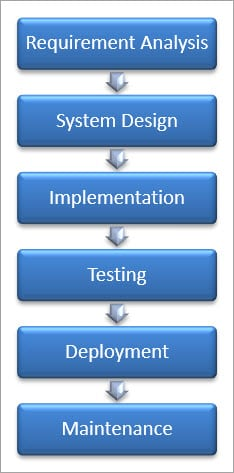
\includegraphics[width=15cm, height=15cm]{water.jpg}
  \caption{Waterfall model}
\end{figure}
\par Waterfall model is the very first model that is used in SDLC. It is also known as the linear sequential model.
In this model, the outcome of one phase is the input for the next phase. Development of the next phase starts only when the previous phase is complete.
\begin{itemize}
    \item Requirement Analysis
    \par First, Requirement gathering and analysis is done. Once the requirement is freeze then only the System Design can start. Here in, the SRS document created is the output for the Requirement phase and it acts as an input for the System Design.
    
    \item System Design
    \par In System Design Software architecture and Design, documents which act as an input for the next phase are created i.e. Implementation and coding.
    \item Implementation 
    \par In the Implementation phase, coding is done and the software developed is the input for next phase i.e. testing.
    
    \item Testing
    \par In the testing phase, the developed code is tested thoroughly to detect the defects in the software. Defects are logged into the defect tracking tool and are retested once fixed. Bug logging, Retest, Regression testing goes on until the time the software is in go-live state.
    
    \item Deployment
    \par In the Deployment phase, the developed code is moved into production after the sign off is given by the customer.
    
    \item Maintainence
    \par Any issues in the production environment are resolved by the developers which come under maintenance.
\chapter{System Design}
\end{itemize}
\section{Mathematical Model}
\textbf{Set Theory Analysis}
Let ‘S’ be the\ding{120} Error detection in big data as the final set S = \{...\}\newline
Identify the inputs as D \newline
D = \{D1, D2, D3, D4 \ding{120} ‘D’ gives data files\}\newline
S = \{D,...\}\newline
L = \{L1, L2 \ding{120} ‘L’ gives the log files for upload and download and repair\}\newline
A = \{A1, A2, A3, \ding{120} ‘A’ gives alerts\}\newline
Identify the functions as ‘F’\newline
S = \{D, L, A, F…\}\newline
F = \{ F1(), F2(), F3(), F4(), F5(), F6() \}\newline
F1 ( V ) :: Upload\newline
F2 ( V) :: integrity check \newline
F3 ( V ) :: Log generation\newlineW
F4 ( T ) :: Sarcasm Detection\newline
F4 ( D ) :: Restore the file\newline
F6 ( V ) :: Download the data file\newline
Identify the outputs as O\newline
S = \{D, L, A, F, O,...\}\newline
Let ‘S’ be the\ding{120}Error detection in big data as the final set S = \{....\}\newline
Identify the inputs as D 
D = \{D1, D2, D3, D4 \ding{120} ‘D’ gives data files\}\newline
S = \{D,...\}\newline
L = \{L1, L2 \ding{120} ‘L’ gives the log files for upload and download and repair\}\newline
A = \{A1, A2, A3, \ding{120} ‘A’ gives alerts\}\newline
Identify the functions as ‘F’\newline
S = \{D, L, A, F,...\}\newline
F = \{ F1(), F2(), F3(), F4(), F5(), F6() \}\newline
F1( V ) :: Upload\newline
F2 ( V) :: integrity check\newline 
F3 ( V ) :: Log generation\newline
F4 ( T ) :: Sarcasm Detection\newline
F4 ( D ) :: Restore the file\newline
F6 ( V ) :: Download the data file\newline
Identify the outputs as O\newline
S = \{D, L, A, F, O,...,\}\newline
\begin{figure}[h!]
  \centering
  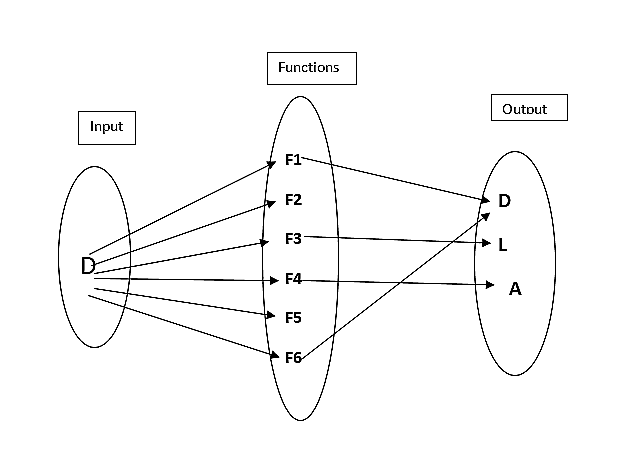
\includegraphics[width=\linewidth]{math.png}
  \caption{Mathematical model: functionality representation}
\end{figure}
\newpage
\section{Data Flow Diagrams}
\begin{figure}[h!]
  \centering
  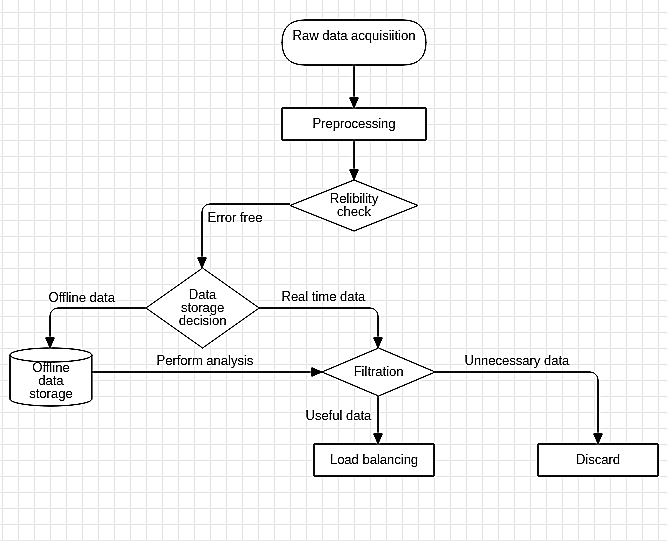
\includegraphics[
  width=13cm,
  height=10cm,
]{dfdl0.png}
  \caption{DFD level 0}
\end{figure}
\textbf{Data Flow Diagram Level 0}
\begin{itemize}
    \item Raw Data Acquisition
    \par Data acquisition is the process of sampling signals that measure real world physical conditions and converting the resulting samples into digital numeric values that can be manipulated by a computer.
    \item Pre-Processing
    \par Data pre-processing is a data mining technique that involves transforming raw data into an understandable format.
    \item Reliability
    \par The data is checked for errors and only reliable data is used for further processing
    \item Data Storage Decision
    \par The data is then checked, The real time data is usually forwarded for filtration process
    \item Offline Data Storage
    \par The offline data is given in the database and then analysis is performed on the data. After the analysis of the offline data, that data is used for filtration. 
    \item Filtration
    \par After filtration, The data which is useful is given for further processing. The un-useful data is discarded
    \item Load Balancing
    \par In Load balancing, the capacity of the system is checked.
\end{itemize}
\begin{figure}[h!]
  \centering
  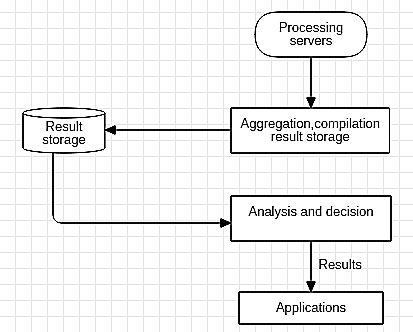
\includegraphics[
  width=13cm,
  height=10cm,
]{dfdl1.png}
  \caption{DFD level 1}
\end{figure}
\newpage 
\textbf{Data Flow Diagram Level 1}
\begin{itemize}
    \item Processing Servers
    \par The data after load balancing is given to the servers for processing, where th actual work of the SDS starts working.
    \item Aggregation, Compilation, Result Storage
    \par Aggregation of attitudes or opinions expressed by internet users towards a specific topic. Analyzing the sentiment of tweets gives an interesting insight into the opinions of the public in relation to a certain event. 
    \item Result Storage 
    \par The data after all the processing is given to the database, where its saved for a temporary period of time.
    \item Analysis and Decision
    \par The data is then analyzed and the decision is made in which the sentence is declared as sarcasm, in a positive, negative and neutral way. And this result is forwarded to the application in a form of an graph.
\end{itemize}
\newpage
\section{UML Diagrams}
\subsection{Block Diagram}
\begin{figure}[h!]
  \centering
  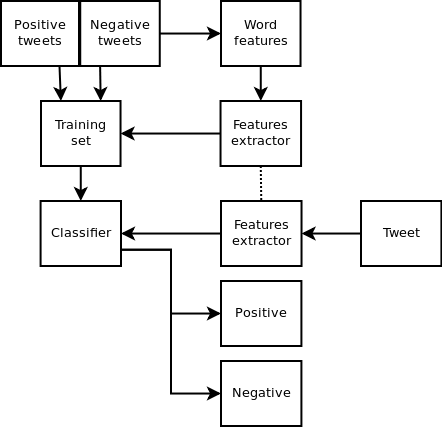
\includegraphics[
  width=13cm,
  height=10cm,
]{block.png}
  \caption{Block diagram}
\end{figure}
\textbf{Block Diagram}
\par Tweet is given to the feature extractor.
\begin{itemize}
    \item Feature Extractor
    \par Feature extraction is an attribute reduction process. Feature extraction starts from an initial set of measured data and builds derived values (features) intended to be informative and non-redundant, facilitating the subsequent learning and generalization steps, and in some cases leading to better human interpretations. Feature extraction is a dimensionality reduction process, where an initial set of raw variables is reduced to more manageable groups (features) for processing, while still accurately and completely describing the original data set.
    \item Classifier 
    The training set created is given to the Classifier. The Classifier on the basis of the probability of the sentence, gives us the sentence classified into two \textbf{Positive} and \textbf{Negative}
\end{itemize}
\subsection{Class Diagram}
\begin{figure}[h!]
  \centering
  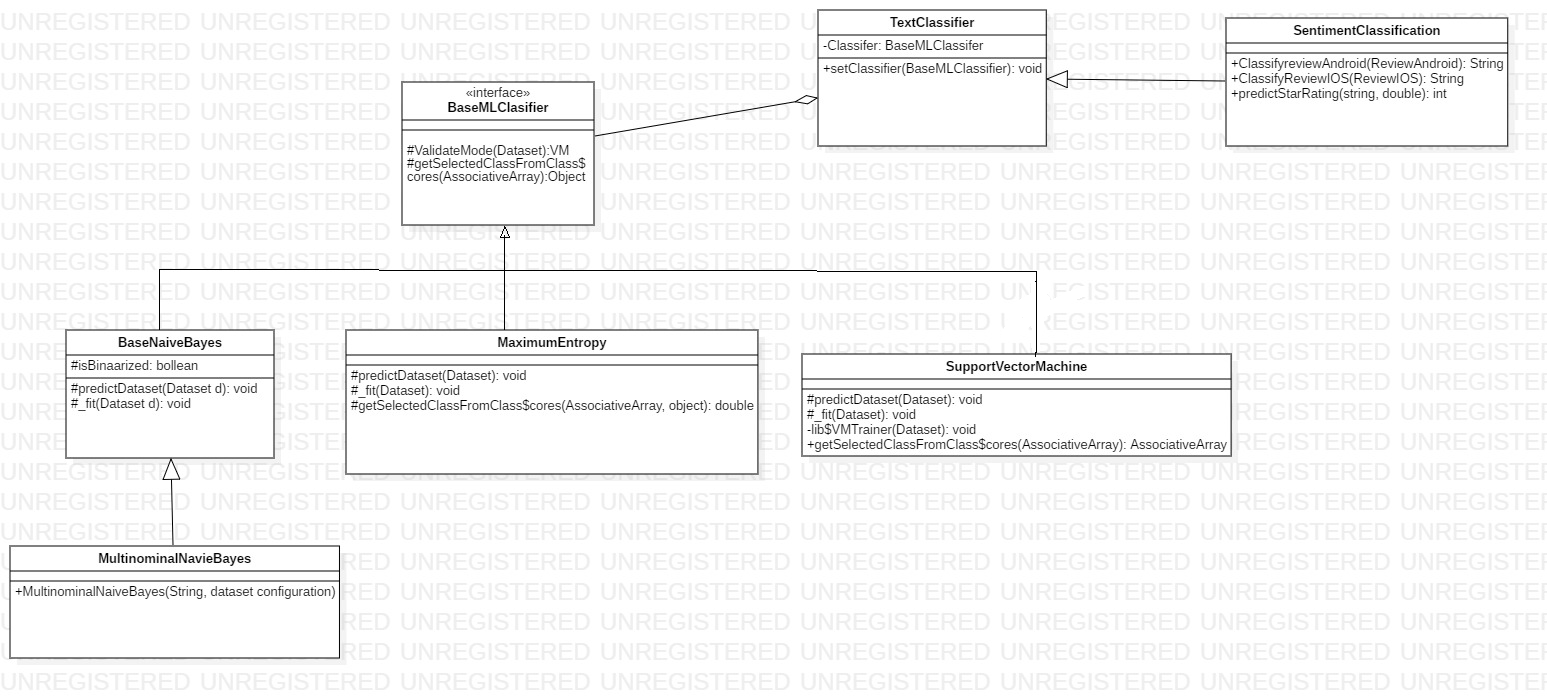
\includegraphics[width=\linewidth]{class.png}
  \caption{Class diagram}
\end{figure}
\begin{itemize}
    \item Text Classifier
    \par Text classification algorithms are at the heart of a variety of software systems that process text data at scale. Email software uses text classifier to determine whether incoming mail is sent to the inbox or filtered into the spam folder.
    \item Naive Bayes
    \par Naive Bayes is among one of the simplest, but most powerful algorithms for classification based on Bayes' Theorem with an assumption of independence among predictors. 
    \par The Naive Bayes classifier assumes that the presence of a feature in a class is unrelated to any other feature. Even if these features depend on each other or upon the existence of the other features, all of these properties independently contribute to the probability that a particular fruit is an apple or an orange or a banana, and that is why it is known as "Naive."
    \par n statistics and probability theory, Bayes' theorem describes the probability of an event, based on prior knowledge of conditions that might be related to the event. It serves as a way to figure out conditional probability.
    Given a Hypothesis (H) and evidence (E), Bayes' Theorem states that the relationship between the probability of the hypothesis before getting the evidence, P(H), and the probability of the hypothesis after getting the evidence, P(H|E), is: \newline
    
    \[p {(H|E)} =\frac{p{(E|H)}.p{(H)}}{p(E)}\]
    
    \item Support Vector Machine
    \par In machine learning, support-vector machines (SVMs, also support-vector networks[1]) are supervised learning models with associated learning algorithms that analyze data used for classification and regression analysis. Given a set of training examples, each marked as belonging to one or the other of two categories, an SVM training algorithm builds a model that assigns new examples to one category or the other, making it a non-probabilistic binary linear classifier (although methods such as Platt scaling exist to use SVM in a probabilistic classification setting). A SVM model is a representation of the examples as points in space, mapped so that the examples of the separate categories are divided by a clear gap that is as wide as possible. New examples are then mapped into that same space and predicted to belong to a category based on which side of the gap they fall.
    \item Maximum Entropy
    \begin{itemize}
        \item Entropy 
        \par is a concept that originated in thermodynamics, and later, via statistical mechanics, motivated entire branches of information theory, statistics, and machine learning.
        \item Maximum entropy
        \par is the state of a physical system at greatest disorder or a statistical model of least encoded information, these being important theoretical analogs.
    \end{itemize}
    \item Sentiment Classification
    \par This classifier determines if a text is positive or negative. It is well suited for both short and long texts (tweets, Facebook statuses, blog posts, product reviews etc)
\end{itemize}
\newpage
\subsection{Activity Diagram}
\begin{figure}[h!]
  \centering
  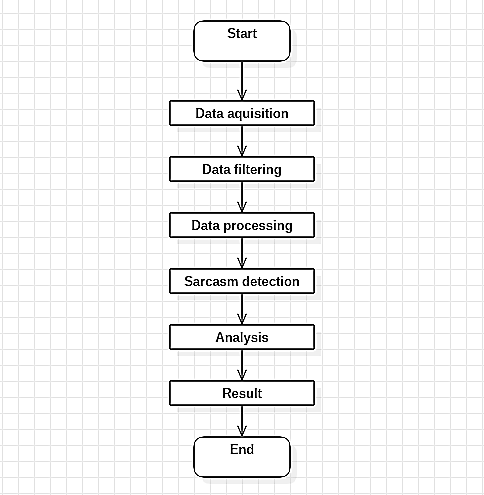
\includegraphics[width=13cm,
  height=10cm]{activity.png}
  \caption{Activity diagram}
\end{figure}
\begin{itemize}
    \item Data Acquisition
    \par Data Acquisition is the process of sampling signals that measure real world physical conditions and converting the resulting samples into digital numeric values that can be manipulated by a computer.
    \item Data Filtering
    \par Cleaning up the text data is necessary to highlight attributes that we’re going to want our machine learning system to pick up on.
     \begin{itemize}
        \item Remove punctuation
        \par Punctuation can provide grammatical context to a sentence which supports our understanding. But for our vectorizer which counts the number of words and not the context, it does not add value, so we remove all special characters. eg: How are you?->How are you
        \item Tokenization
        \par Tokenizing separates text into units such as sentences or words. It gives structure to previously unstructured text. eg: Plata o Plomo-> ‘Plata’,’o’,’Plomo’.
        \item Remove stopwords
        \par Stopwords are common words that will likely appear in any text. They don’t tell us much about our data so we remove them. eg: silver or lead is fine for me-> silver, lead, fine.
    \end{itemize}
    \item Data Processing
    \begin{itemize}
        \item Stemming
        \par Stemming helps reduce a word to its stem form. It often makes sense to treat related words in the same way. It removes suffices, like “ing”, “ly”, “s”, etc. by a simple rule-based approach. It reduces the corpus of words but often the actual words get neglected. eg: Entitling,Entitled->Entitl
        \item Lemmatizing
        \par Lemmatizing derives the canonical form (‘lemma’) of a word. i.e the root form. It is better than stemming as it uses a dictionary-based approach i.e a morphological analysis to the root word.eg: Entitling, Entitled->Entitle
        \item Vectorizing Data
        \par Vectorizing is the process of encoding text as integers i.e. numeric form to create feature vectors so that machine learning algorithms can understand our data.
    \end{itemize}
    \item Sarcasm Detection
    \par sarcasm detection is the task of predicting sarcasm in text. 
    \item Results
    \par In the form of a graph, the sentences would be shown as either positive, negative and neutral
\end{itemize}
\newpage
\subsection{Sequence Diagram}
\begin{figure}[h!]
  \centering
  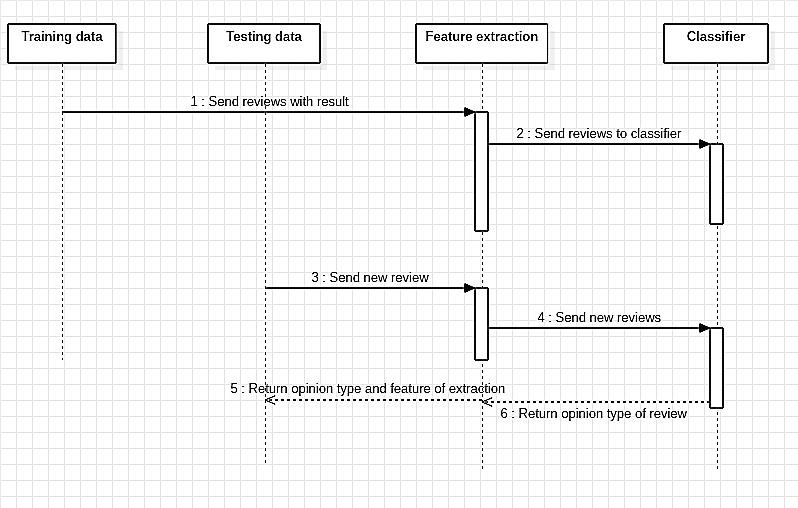
\includegraphics[width=15cm,
  height=13cm]{sequence.png}
  \caption{Sequence diagram}
\end{figure}
\begin{itemize}
    \item Training Set
    \par The data is send with results. After the process of feature extracion of the data, the original data set is copied into the training dataset.
    \item Testing Set
    \par The data set on which the processing is performed.
    \item Feature Extraction
    \par After the feature of the data is extracted, the data is sent to the classifier
    \item Classifier
    \par The classifier sends an opinion of the data.
\end{itemize}
\subsection{Use Case Diagram}
\begin{figure}[h!]
  \centering
  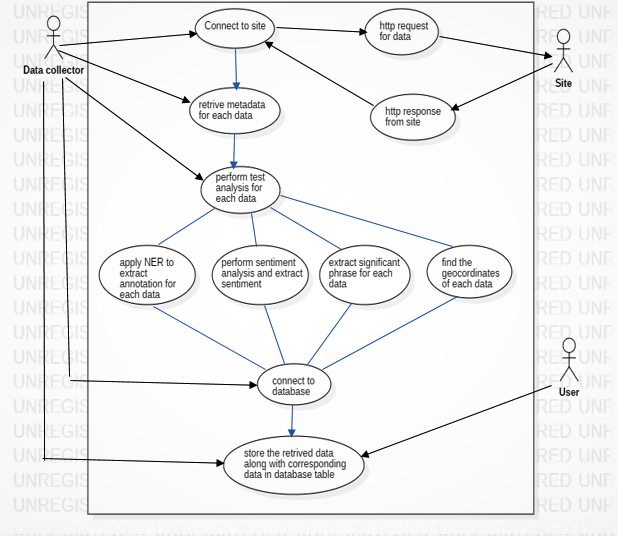
\includegraphics[width=15cm,
  height=13cm]{usecase.png}
  \caption{Use case diagram}
\end{figure}
\begin{itemize}
    \item Data Collector
    \begin{itemize}
        \item Connects to Site
        \item Retrieve Metadata
        \item Performs Test Analysis
        \item Connect to databases
        \item Stores the retrieved Data
    \end{itemize}
    \item Site
    \par Gives http response to the data collector.
    \item User
    \par Stores the retrieved Data along with corresponding data in database tables.
\end{itemize}
\chapter{Project Plan}
\section{Project Estimate}
\subsection{Reconciled Estimates}
\subsubsection{Planning phase}
\begin{center}
 \begin{tabular}{||c || c ||} 
 \hline
 Month & Plan \\ [1.5ex] 
 \hline\hline
 June & Domain Selection \\ 
 \hline
 July & Title Finalization \\
 \hline
 August & Technology Selection \\ [1.5ex]
 \hline
\end{tabular}
\end{center}
\subsubsection{Implementation phase}
\begin{center}
 \begin{tabular}{||c || c ||} 
 \hline
 Month & Plan \\ [1.5ex] 
 \hline\hline
 September & Literature Survey \\ 
 \hline
 October & Report and UML \\
 \hline
 November & Presentation \\
 \hline
  December & Paper Writing \\ 
 \hline
 January & Module 1 (Data Acquisition), Module 2(Data Filtering)\\
 \hline
 February & Module 3 (Data Analysis) \\
 \hline
 March & Module 4 (Prediction) \\ 
 \hline
 April & Module 5 (Data Storage) \\
 \hline
 May & Final Project Execution \\ [1.5ex]
 \hline
\end{tabular}
\end{center}
\subsection{Project Resources}
\section{Risk Management}
This section discusses Project risks and the approach to managing them.
\begin{itemize}
    \item Easy data ingestion:
    \par  Copying data to and from the cloud  is as simple as copying data to a standard file system using Direct Access NFS. Applications can therefore ingest data into the cloud server in real time without any staging areas or separate clusters just to ingest data.
    \item Existing applications work: 
    \par Due to the UNIX platform's PO SIX compliance, any python application works directly on cloud without undergoing code changes. Existing tool sets, custom utilities and applications are good to go on day one
    \item Multi-tenancy:
    \par Support multiple user groups, any and all enterprise data sets, and multiple applications in the same cluster. Data modellers, developers and analysts can all work in unison on the same cluster without stepping on each others toes.
    \item Business continuity:
    \par  cloud provides integrated high availability (HA), data protection, and disaster recovery (DR) capabilities to protect against both hardware failure as well as site-wide failure.
    \item High scalability:
    \par  Scalability is key to bringing all data together on one platform so the analytics are much more nuanced and accurate. cloud is the only platform that scales all the way to a trillion files without compromising performance.
    \item High performance:
    \par  The Distribution for cloud was designed for high performance, with respect to both high throughput and low latency. In addition, a fraction of servers are required for running cloud distributions, leading to architectural simplicity and lower capital and operational expenses.
\end{itemize}
\subsection{Risk Identification}
\begin{itemize}
    \item Security Information and Event Management (SIEM): 
    \par Analyze and correlate large amounts of real-time data from network and security devices to manage external and internal security threats, improve incident response time and compliance reporting.
    \item Application Log Monitoring:
    \par Improve analysis of application log data to better manage system resource utilization, security issues, and diagnose and pre-empt production application problems.
    \item Network Intrusion Detection:
    \par Monitor and analyze network traffic to detect, identify, and report on suspicious activity or intruders.
    \item Fraud Detection:
    \par Use pattern/anomaly recognition on larger volumes and variety of data to detect and prevent fraudulent activities by external or internal parties.
    \item Risk Modelling:
    \par Improve risk assessment and associated scoring by building sophisticated machine learning models on cloud that can take into account hundreds or even thousands of indicators.
\end{itemize}
\subsection{Risk Analysis}
The risks for the Project can be analyzed within the constraints of time and quality
\begin{center}
    \begin{table}[H]
\centering
\begin{tabular}{||c||c||c||c||c||c||}
%row no:1
\multicolumn{1}{c}{\begin{tabular}{c}ID\\\end{tabular}} & 
\multicolumn{1}{c}{\begin{tabular}{c}Risk Description\\\end{tabular}} & 
\multicolumn{1}{c}{\begin{tabular}{c}Probability\\\end{tabular}} & 
\multicolumn{3}{c}{Impact} \\
\hline
\hline
%row no:2
\multicolumn{1}{c}{} & 
\multicolumn{1}{c}{} & 
\multicolumn{1}{c}{} & 
\multicolumn{1}{c}{Schedule} & 
\multicolumn{1}{c}{Quality} & 
\multicolumn{1}{c}{Overall} \\
\hline
\hline
%row no:3
\multicolumn{1}{p{0.16in}}{1} & 
\multicolumn{1}{p{1.87in}}{Security Information and Event Management (SI EM)} & 
\multicolumn{1}{p{0.78in}}{Low} & 
\multicolumn{1}{p{0.61in}}{Low} & 
\multicolumn{1}{p{0.47in}}{Low} & 
\multicolumn{1}{p{0.48in}}{Low} \\
\hline
\hline
%row no:4
\multicolumn{1}{p{0.16in}}{2} & 
\multicolumn{1}{p{1.87in}}{Application Log Monitoring} & 
\multicolumn{1}{p{0.78in}}{High} & 
\multicolumn{1}{p{0.61in}}{High} & 
\multicolumn{1}{p{0.47in}}{High} & 
\multicolumn{1}{p{0.48in}}{High} \\
\hline
\hline
%row no:5
\multicolumn{1}{p{0.16in}}{3} & 
\multicolumn{1}{p{1.87in}}{Network Intrusion Detection} & 
\multicolumn{1}{p{0.78in}}{Low} & 
\multicolumn{1}{p{0.61in}}{High} & 
\multicolumn{1}{p{0.47in}}{Low} & 
\multicolumn{1}{p{0.48in}}{Low} \\
\hline
\hline
%row no:6
\multicolumn{1}{p{0.16in}}{4} & 
\multicolumn{1}{p{1.87in}}{Fraud Detection} & 
\multicolumn{1}{p{0.78in}}{Low} & 
\multicolumn{1}{p{0.61in}}{Low} & 
\multicolumn{1}{p{0.47in}}{Low} & 
\multicolumn{1}{p{0.48in}}{Low} \\
\hline
\hline
%row no:7
\multicolumn{1}{p{0.16in}}{5} & 
\multicolumn{1}{p{1.87in}}{Risk Modeling} & 
\multicolumn{1}{p{0.78in}}{High} & 
\multicolumn{1}{p{0.61in}}{High} & 
\multicolumn{1}{p{0.47in}}{High} & 
\multicolumn{1}{p{0.48in}}{High} \\
\hline
\hline

\end{tabular}
\caption{Risk table}
\end{table}
\end{center}
%-------------------------------------------------
\begin{table}[H]
 			\centering
\begin{tabular}{|| p || p|| p|| }
\hline
\hline
%row no:1
\multicolumn{1}{p{0.71in}}{Probability} & 
\multicolumn{1}{p{1.81in}}{Value} & 
\multicolumn{1}{p{0.75in}}{Description} \\
\hline
\hline
%row no:2
\multicolumn{1}{p{0.71in}}{High} & 
\multicolumn{1}{p{1.81in}}{Probability of occurrence is} & 
\multicolumn{1}{p{0.75in}}{\textit{$ > $} 75$\%$ } \\
\hline
\hline
%row no:3
\multicolumn{1}{p{0.71in}}{Medium} & 
\multicolumn{1}{p{1.81in}}{Probability of occurrence is} & 
\multicolumn{1}{p{0.75in}}{26 \textit{$-$}75$\%$ } \\
\hline
\hline
%row no:4
\multicolumn{1}{p{0.71in}}{Low} & 
\multicolumn{1}{p{1.81in}}{Probability of occurrence is} & 
\multicolumn{1}{p{0.75in}}{\textit{$<$} 25$\%$ } \\
\hline
\hline
\end{tabular}
\caption{Risk probability definitions}
 \end{table}
 %-----------------------------------------------
 \begin{center}
     \begin{table}[H]
\centering
\begin{tabular}{p{0.62in}p{0.53in}p{3.81in}}
%row no:1
\hline
\hline
\multicolumn{1}{p{0.62in}}{Impact} & 
\multicolumn{1}{p{0.53in}}{Value} & 
\multicolumn{1}{p{3.81in}}{Description} \\
\hline
\hline
%row no:2
\multicolumn{1}{p{0.62in}}{Medium} & 
\multicolumn{1}{p{0.53in}}{\textit{$<$}5$\%$ } & 
\multicolumn{1}{p{3.81in}}{Schedule impact or Barely noticeable degradation in qual- ity Low Impact on schedule or Quality can be incorporated} \\
\hline
\hline
%row no:3
\multicolumn{1}{p{0.62in}}{High} & 
\multicolumn{1}{p{0.53in}}{5 \textit{$-$  }10$\%$ } & 
\multicolumn{1}{p{3.81in}}{Schedule impact or Some parts of the project have low quality} \\
\hline
\hline
%row no:4
\multicolumn{1}{p{0.62in}}{Very high} & 
\multicolumn{1}{p{0.53in}}{\textit{$>$}10$\%$ } & 
\multicolumn{1}{p{3.81in}}{Schedule impact or Unacceptable quality} \\
\hline
\hline
\end{tabular}
\caption{Risk impact definitions}
\end{table}
\end{center}
%---------------------------------------------------------------
Following are the details for each risk.
\begin{table}[H]
\centering
\begin{tabular}{p{1.09in} p{4.07in}}
%row no:1
\hline
\hline
\multicolumn{1}{p{1.09in}}{Risk ID} & 
\multicolumn{1}{p{4.07in}}{1} \\
\hline
\hline
%row no:2
\multicolumn{1}{p{1.09in}}{Risk Description} & 
\multicolumn{1}{p{4.07in}}{Analyze and correlate large amounts of real-time data from network and security devices to manage external and internal security threats, improve incident response time and compliance reporting.} \\
\hline

%row no:3
\multicolumn{1}{p{1.09in}}{Category} & 
\multicolumn{1}{p{4.07in}}{Security Information and Event Management.} \\
\hline

%row no:4
\multicolumn{1}{p{1.09in}}{Source} & 
\multicolumn{1}{p{4.07in}}{Cloud Cluster} \\
\hline

%row no:5
\multicolumn{1}{p{1.09in}}{Probability} & 
\multicolumn{1}{p{4.07in}}{Low} \\
\hline

%row no:6
\multicolumn{1}{p{1.09in}}{Impact} & 
\multicolumn{1}{p{4.07in}}{Low} \\
\hline

%row no:7
\multicolumn{1}{p{1.09in}}{Response} & 
\multicolumn{1}{p{4.07in}}{Mitigate} \\
\hline

%row no:8
\multicolumn{1}{p{1.09in}}{Strategy} & 
\multicolumn{1}{p{4.07in}}{High Performance} \\

\hline
%row no:9
\multicolumn{1}{p{1.09in}}{Risk Status} & 
\multicolumn{1}{p{4.07in}}{Rarely Occurred} \\
\hline
\hline
\end{tabular}
\caption{Risk description for ID 1}
\end{table}
%-----------------------------------------------------------
\begin{center}
\begin{table}[H]
\centering
\begin{tabular}{p{1.09in}p{4.07in}}
%row no:1
\hline
\hline
\multicolumn{1}{p{1.09in}}{Risk ID} & 
\multicolumn{1}{p{4.07in}}{2} \\
\hline
\hline
%row no:2
\multicolumn{1}{p{1.09in}}{Risk Description} & 
\multicolumn{1}{p{4.07in}}{Improve analysis of application log data to better manage system resource utilization, security issues, and diagnose and preempt production application problems. \par } \\
\hline
%row no:3
\multicolumn{1}{p{1.09in}}{Category} & 
\multicolumn{1}{p{4.07in}}{Application Log Monitoring} \\
\hline
%row no:4
\multicolumn{1}{p{1.09in}}{Source} & 
\multicolumn{1}{p{4.07in}}{Processing Server} \\
\hline
%row no:5
\multicolumn{1}{p{1.09in}}{Probability} & 
\multicolumn{1}{p{4.07in}}{High} \\
\hline
%row no:6
\multicolumn{1}{p{1.09in}}{Impact} & 
\multicolumn{1}{p{4.07in}}{High} \\
\hline
%row no:7
\multicolumn{1}{p{1.09in}}{Response} & 
\multicolumn{1}{p{4.07in}}{Continuous} \\
\hline
%row no:8
\multicolumn{1}{p{1.09in}}{Strategy} & 
\multicolumn{1}{p{4.07in}}{Multi Tenancy} \\
\hline
%row no:9
\multicolumn{1}{p{1.09in}}{Risk Status} & 
\multicolumn{1}{p{4.07in}}{Occurred} \\
\hline
\hline
\end{tabular}
\caption{Risk description for ID 2}
\end{table}
%---------------------------------------------------------------------------------------
\begin{table}[H]
\centering
\begin{tabular}{p{1.09in}p{4.07in}}
%row no:1
\hline
\hline
\multicolumn{1}{p{1.09in}}{Risk ID} & 
\multicolumn{1}{p{4.07in}}{3} \\
\hline
\hline
%row no:2
\multicolumn{1}{p{1.09in}}{Risk Description} & 
\multicolumn{1}{p{4.07in}}{Monitor and analyze network traffic to detect, identify, and report on suspicious activity or intruders. \par } \\
\hline
%row no:3
\multicolumn{1}{p{1.09in}}{Category} & 
\multicolumn{1}{p{4.07in}}{Network Intrusion Detection} \\
\hline
%row no:4
\multicolumn{1}{p{1.09in}}{Source} & 
\multicolumn{1}{p{4.07in}}{NameNode} \\
\hline
%row no:5
\multicolumn{1}{p{1.09in}}{Probability} & 
\multicolumn{1}{p{4.07in}}{Low} \\
\hline
%row no:6
\multicolumn{1}{p{1.09in}}{Impact} & 
\multicolumn{1}{p{4.07in}}{Low} \\
\hline
%row no:7
\multicolumn{1}{p{1.09in}}{Response} & 
\multicolumn{1}{p{4.07in}}{Mitigate} \\
\hline
%row no:8
\multicolumn{1}{p{1.09in}}{Strategy} & 
\multicolumn{1}{p{4.07in}}{High Scalability} \\
\hline
%row no:9
\multicolumn{1}{p{1.09in}}{Risk Status} & 
\multicolumn{1}{p{4.07in}}{Identified} \\
\hline
\hline
\end{tabular}
\caption{Risk description for ID 3}
\end{table}
%--------------------------------------------------------------------
\begin{table}[H]
\centering
\begin{tabular}{p{1.09in}p{4.07in}}
%row no:1
\hline
\hline
\multicolumn{1}{p{1.09in}}{Risk ID} & 
\multicolumn{1}{p{4.07in}}{4} \\
\hline
%row no:2
\multicolumn{1}{p{1.09in}}{Risk Description} & 
\multicolumn{1}{p{4.07in}}{Use pattern/anomaly recognition on larger volumes and variety of data to detect and prevent fraudulent activities by external or internal parties. \par } \\
\hline
%row no:3
\multicolumn{1}{p{1.09in}}{Category} & 
\multicolumn{1}{p{4.07in}}{Fraud Detection} \\
\hline
%row no:4
\multicolumn{1}{p{1.09in}}{Source} & 
\multicolumn{1}{p{4.07in}}{Web Server - API} \\
\hline
%row no:5
\multicolumn{1}{p{1.09in}}{Probability} & 
\multicolumn{1}{p{4.07in}}{Low} \\
\hline
%row no:6
\multicolumn{1}{p{1.09in}}{Impact} & 
\multicolumn{1}{p{4.07in}}{Low} \\
\hline
%row no:7
\multicolumn{1}{p{1.09in}}{Response} & 
\multicolumn{1}{p{4.07in}}{Mitigate} \\
\hline
%row no:8
\multicolumn{1}{p{1.09in}}{Strategy} & 
\multicolumn{1}{p{4.07in}}{Easy Data Ingestion} \\
\hline
%row no:9
\multicolumn{1}{p{1.09in}}{Risk Status} & 
\multicolumn{1}{p{4.07in}}{Identified} \\
\hline
\hline
\end{tabular}
\caption{Risk description for ID 4}
\end{table}
%---------------------------------------------------------------------------
\begin{table}[H]
\centering
\begin{tabular}{p{1.09in}p{4.07in}}
%row no:1
\hline
\hline
\multicolumn{1}{p{1.09in}}{Risk ID} & 
\multicolumn{1}{p{4.07in}}{5} \\
\hline
%row no:2
\multicolumn{1}{p{1.09in}}{Risk Description} & 
\multicolumn{1}{p{4.07in}}{Improve risk assessment and associated scoring by building sophisticated machine learning models on Hadoop that can take into account hundreds or even thousands of indicators.} \\
\hline
%row no:3
\multicolumn{1}{p{1.09in}}{Category} & 
\multicolumn{1}{p{4.07in}}{Risk Modeling} \\
\hline
%row no:4
\multicolumn{1}{p{1.09in}}{Source} & 
\multicolumn{1}{p{4.07in}}{Client Interface} \\
\hline
%row no:5
\multicolumn{1}{p{1.09in}}{Probability} & 
\multicolumn{1}{p{4.07in}}{High} \\
\hline
%row no:6
\multicolumn{1}{p{1.09in}}{Impact} & 
\multicolumn{1}{p{4.07in}}{High} \\
\hline
%row no:7
\multicolumn{1}{p{1.09in}}{Response} & 
\multicolumn{1}{p{4.07in}}{Continuous} \\
\hline
%row no:8
\multicolumn{1}{p{1.09in}}{Strategy} & 
\multicolumn{1}{p{4.07in}}{Existing Application Work.} \\
\hline
%row no:9
\multicolumn{1}{p{1.09in}}{Risk Status} & 
\multicolumn{1}{p{4.07in}}{Occurred} \\
\hline
\hline
\end{tabular}
\caption{Risk description for ID 5}
\end{table}
\end{center}
%---------------------------------------------------------------------------
\subsection{Overview of Risk Mitigation, Monitoring, Management}
\subsubsection{Risk Mitigation}
The ultimate purpose of risk identification and analysis is to prepare for risk mitigation. Mitigation includes reduction of the likelihood that a risk event will occur and/or reduction of the effect of a risk event if it does occur. This chapter discusses the importance of risk mitigation planning and describes approaches to reducing or mitigating project risks.
\begin{itemize}
    \item RISK MITIGATION PLANNING
    \par
Risk management planning needs to be an ongoing effort that cannot stop after a qualitative risk assessment, or a Monte Carlo simulation, or the setting of contingency levels. Risk management includes front-end planning of how major risks will be mitigated and managed once identified. Therefore, risk mitigation strategies and specific action plans should be incorporated in the project execution plan, or risk analyses are just so much wallpaper. Risk mitigation plans should
\begin{itemize}
    \item Characterize the root causes of risks that have been identified and quantified in earlier phases of the risk management process.
    \item Evaluate risk interactions and common causes.
    \item Identify alternative mitigation strategies, methods, and tools for each major risk.
    \item Assess and prioritize mitigation alternatives.
\end{itemize}
Although risk mitigation plans may be developed in detail and executed by contractors, the owner’s program and project management should develop standards for a consistent risk mitigation planning process. Owners should have independent, unbiased outside experts review the project’s risk mitigation plans before final approval. This should be done prior to completing the project design or allocating funds for construction. Risk mitigation planning should continue beyond the end of the project by capturing data and lessons learned that can benefit future projects.
\item RISK RESPONSE AND MITIGATION TOOLS
\par 
Some risks, once identified, can readily be eliminated or reduced. However, most risks are much more difficult to mitigate, particularly high-impact, low-probability risks. Therefore, risk mitigation and management need to be long-term efforts by project directors throughout the project.
\begin{itemize}
    \item Responding to the Level of Uncertainty
    \item Dealing With High-Impact, Low-Probability Risks
    \item Risk Transfer and Contracting
    \item Risk Buffering
    \item Risk Avoidance
    \item Risk Control
    \item Organizational Flexibility
\end{itemize}
\end{itemize}
\subsubsection{Risk Monitoring}
Risk monitoring is the ongoing process of managing risk. Risk management often has an initial phase that involves identifying risk, agreeing to treatments and designing controls. Risk monitoring is the process of tracking risk management execution and continuing to identify and manage new risks. The following are common elements of risk monitoring.
\begin{itemize}
    \item Risk Identification
    \item Risk Analysis
    \item Risk Controls
    \item Measurement & Communication
\end{itemize}
\subsubsection{Risk Management}
Risk management means risk containment and mitigation. First, you’ve got to identify and plan. Then be ready to act when a risk arises, drawing upon the experience and knowledge of the entire team to minimize the impact to the project. 
Risk management includes the following tasks:
\begin{itemize}
    \item \textbf{Identify} risks and their triggers
    \item \textbf{Classify} and prioritize all risks
    \item Craft a \textbf{plan} that links each risk to a mitigation
    \item \textbf{Monitor} for risk triggers during the project
    \item Implement the \textbf{mitigating action} if any risk materializes
    \item \textbf{Communicate} risk status throughout project
\end{itemize}
\section{Project Schedule}
\subsection{Project Task Set}
Major Task in the Project stages are:
\begin{table}[ht]
    \centering
    \large
     \begin{tabular}{ | p{3.7cm} | p{10cm} |}
    \hline
    Dates  & 	Task \\\hline
     & 	Domain Selection \\ \hline
     & 	Topic Finalization \\ \hline
     &	Feasibility Study and Market Analysis \\ \hline
     &  Abstract Submission \\ \hline
     &	System Architecture Design \\ \hline
     &	Discussion about Platform Issues \\ \hline
     &	Preparing Synopsis \\ \hline
     &	Project Report Submission for Stage 1 \\ \hline
     &  Discussion about Platform Selection \\ \hline
    January 2019 &	System Design and Coding \\ \hline
    February 2019 &	Design and Coding \\ \hline
    March 2019 &	Testing \\ \hline
    April 2019 &	Final Report Preparation \\ \hline
    \end{tabular}
    \caption{Project stages}
\end{table}
\subsection{Task Network}
\begin{figure}[h]
\begin{center}
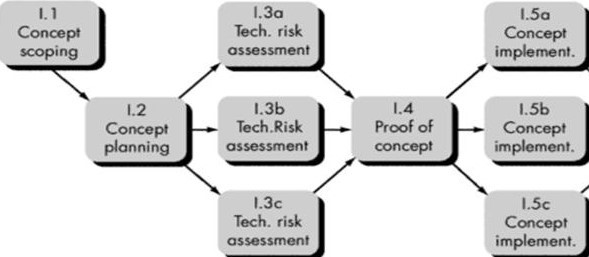
\includegraphics[scale=0.8]{tasks.jpg}
\caption{Task network}
\end{center}
\end{figure}
\subsection{Time line Chart}
\begin{figure}[h!]
  \centering
  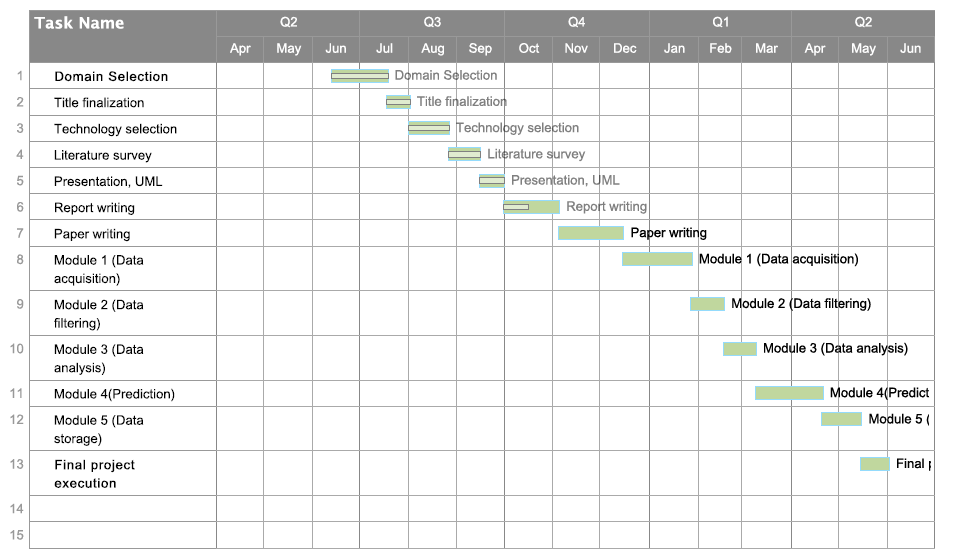
\includegraphics[width=15cm,
  height=13cm]{gnattchart.png}
  \caption{Gnatt chart}
\end{figure}
\section{Team Organization}
\subsection{Team structure}
\begin{itemize}
    \item There are 5 members in our group among them 4 are students which will coordinate with each other and do the survey , implementation and presentation of the project under the guidance of the 5th member(Guide).
    \item The project is evenly divided among the 4 members of the group so that each one of us can work equally ,interactively ,and smartly under the guidance of our project leader(Guide).
\end{itemize}

The team structure for the project is as follows

\begin{itemize}
    \item \textbf{Group 1 :} 1 member has worked on data collection.
    \item \textbf{Group 2 :} 2 members have worked on the Database Management and Backend 
    \item \textbf{Group 3 :} 1 member has worked on front end and Documentation
\end{itemize}
\subsection{Management reporting and communication}
\begin{itemize}
    \item All task were divided evenly and distributed with full coordination among the members.
    \item Periodic Assessment was prepared and accordingly were reported the guide gor validation.
    \item All the reporting intra  as well as inter communication were performed sequentially thus enabling a smooth transaction in developing and executing the proposed project successfully.
\end{itemize}
\chapter{Project Implementation}
\section{Overview of Project Modules}
\textbf{Proposed System}
In our proposed system for analyzing real time as well as offline data for real-time applications using term Big Data we have divided real time Big Data processing architecture into three parts, i.e., 1) Data Acquisition Unit 2) Data Processing Unit and 3) Data Analysis and Decision Unit. In these three unit various algorithms or techniques will be implied on data for it’s analysis. The functionalities and working of three units is as explained and shown in diagram below:
\begin{figure}[h!]
  \centering
  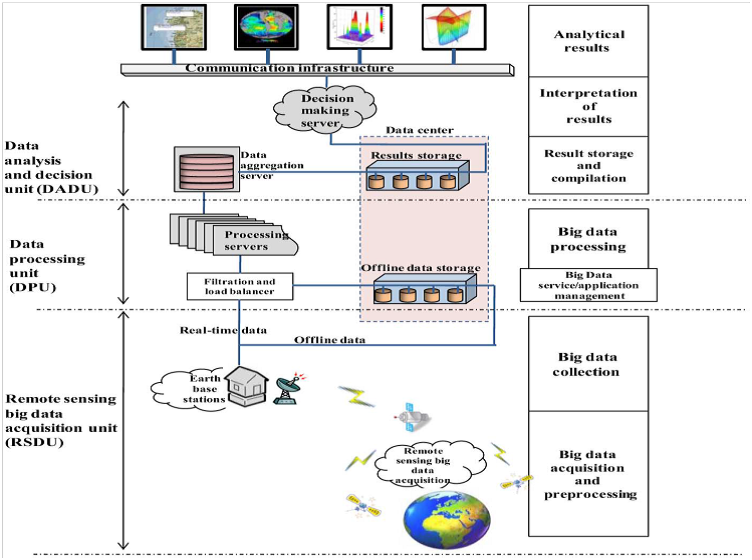
\includegraphics[width=15cm,
  height=13cm]{bdaf.png}
  \caption{Big data analytical framework}
\end{figure}
\textbf{Data  Acquisition Unit}:
\par The need for parallel processing of the massive volume of data was required, which could efficiently analyze the Big Data. For that reason, the proposed unit is introduced in the real time Big Data processing framework that gathers the massive volume of data from various available data gathering unit around the world. We assume that the data capturing unit can correct the erroneous data. For effective data analysis, the Base System pre-processes data under many situations to integrate the data from different sources, which not only decreases storage cost, but also improves analysis accuracy. Some relational data pre-processing techniques are data integration, data cleaning, and redundancy elimination. The data must be corrected in different methods to remove distortions caused due to the motion of the platform. We divided the data processing procedure into two steps, such as real-time Big Data processing and offline Big Data processing. In the case of offline data processing, the Base System transmits the data to the data centre for storage. This data is then used for future analyses. However, in real-time data processing, the data are directly transmitted to the filtration and load balancer server, since storing of incoming real-time data degrades the performance of real-time processing.
\newline 
\textbf{Data Processing Unit}
\par In data processing unit, has two basic functionalities filtration and load balancer. Filtration mainly involves filtration of data and load balancing of processing power. Filtration makes process of filtering data which is useful to us for analysis and blocks other data. It will surely help to improve performance of system as we are only dealing with the useful data. Load balancer is part of server it will provide a provision of dividing data into parts and assign them to the various processing servers. The filtration and load-balancing algorithm varies from analysis to analysis. Each processing server has its own algorithm implementation for processing incoming segment of data from load balancer. Each processing server makes statistical calculations, any measurements, and performs other mathematical or logical tasks to generate intermediate results against each segment of data. These tasks are performed parallel and independently such that the performance of system is increased at an extent and result segments are generated in real time. The results generated by each server are then sent to the aggregation server for compilation, organization, and storing for further processing.
\textbf{Data Analysis and Decision}
\par This unit contains three major functions, such as aggregation and compilation server, results storage server, and decision making server. When results are to be send to the compilation the data is not in aggregated form. So it is necessary to make the given data in aggregated form for proper storage and processing. In this unit many aggregation algorithms are implied so that organized results are stored into the storage. The aggregation server also sends the same copy of that result to the decision-making server to process that result for making decision. The aggregation server also sends the same copy of that result to the decision-making server to process that result for making decision.
\begin{figure}[h!]
  \centering
  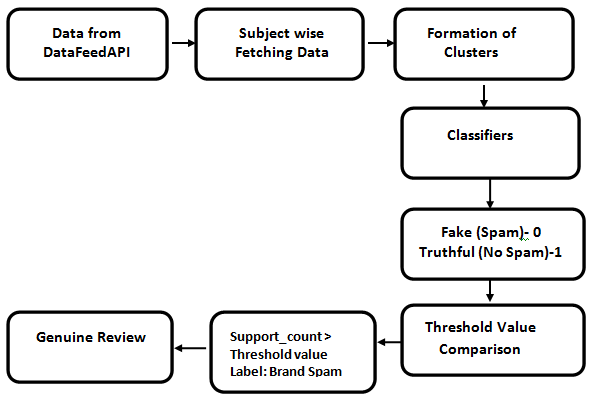
\includegraphics[width=15cm,
  height=13cm]{system.png}
  \caption{Framework process}
\end{figure}
\subsubsection{ Research Hypothesis}
\par Proposed system will easily collect and aggregate the large amount of real-time data. Also the proposed system will be able to make effective processing on collected information and will discard the unused data by various methods so that we can have only the which we want to analyze. Also proposed system will be capable of giving accurate results on the data analysis and will give effective decisions based on them. System will improve the accuracy as well as the quality of the results produced. It will be convenient than traditional analysis systems.
\begin{itemize}
    \item Real-Time Applications
    \par Real-time applications like many social media applications generate massive information. Effective analysis is necessary to have better analysis. Big data analytics helps to have better analysis based on the analysis accurate results and decisions.
    \item Business
    \par Customer Feedback, trends etc.
    \item Health
    \par Health care organizations are leveraging big data technology to capture all the information about a patient to get more complete view for insight into care coordination, health management outcome. Use of big data helps to build a sustainable health care system increase the access to health care.
    \item  Energy utility
    \par Big data can also be the key to actually deploying condition based maintenance program and improve forecasting and scheduling of assets.
\end{itemize}
\section{Tools and Technologies Used}
\subsection{Natural Language Processing}
\textbf{NLP} is a field that covers computer understanding and manipulation of human language, and it’s ripe with possibilities for news gathering. NLP is a way for computers to analyze, understand, and derive meaning from human language in a smart and useful way. By utilizing NLP, developers can organize and structure knowledge to perform tasks such as automatic summarization, translation, named entity recognition, relationship extraction, sentiment analysis, speech recognition, and topic segmentation.

\subsubsection{Basic Terminologies}
\begin{itemize}
    \item Morphology
    It is a study of construction of words from primitive meaningful units.
    \item Syntax
    It refers to arranging words to make a sentence. It also involves determining the structural role of words in the sentence and in phrases.
    \item Semantics
    It is concerned with the meaning of words and how to combine words into meaningful phrases and sentences.
    \item Pragmatics
    It deals with using and understanding sentences in different situations and how the interpretation of the sentence is affected.
    \item Discourse
    It deals with how the immediately preceding sentence can affect the interpretation of the next sentence.
\end{itemize}
\begin{figure}[h!]
  \centering
  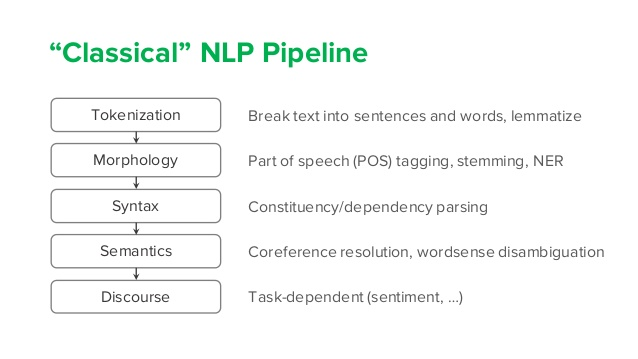
\includegraphics[width=\linewidth]{nlp.png}
  \caption{NLP}
\end{figure}
\newpage
\subsubsection{Steps in NLP}
\begin{itemize}
    \item Lexical Analysis
    It involves identifying and analyzing the structure of words. Lexicon of a language means the collection of words and phrases in a language. Lexical analysis is dividing the whole chunk of txt into paragraphs, sentences, and words.
    \item Syntactic Analysis (Parsing)
    It involves analysis of words in the sentence for grammar and arranging words in a manner that shows the relationship among the words. The sentence such as “The school goes to boy” is rejected by English syntactic analyzer.
    \item Semantic Analysis
    It draws the exact meaning or the dictionary meaning from the text. The text is checked for meaningfulness. It is done by mapping syntactic structures and objects in the task domain. The semantic analyzer disregards sentence such as “hot ice-cream”.
    \item Disclosure Integration
    The meaning of any sentence depends upon the meaning of the sentence just before it. In addition, it also brings about the meaning of immediately succeeding sentence.
    \item Pragmatic Analysis
    During this, what was said is re-interpreted on what it actually meant. It involves deriving those aspects of language which require real world knowledge.
\end{itemize}
\begin{figure}[h!]
  \centering
  %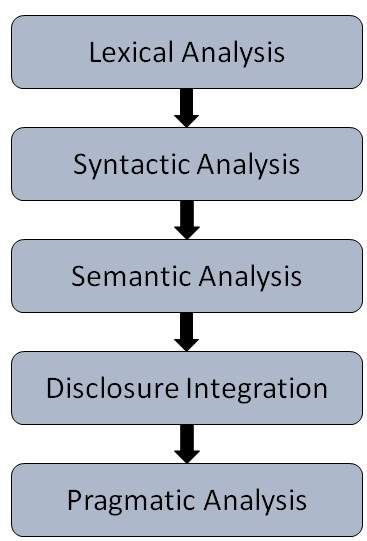
\includegraphics[width=\linewidth]{nlpstep.png}
  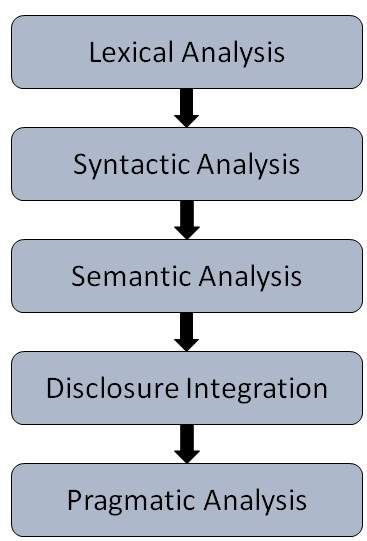
\includegraphics[
  width=13cm,
  height=10cm,
]{nlpstep.png}
  \caption{Steps in NLP}
\end{figure}
\newpage
\subsubsection{Text Factorization}
\begin{figure}[h!]
  \centering
  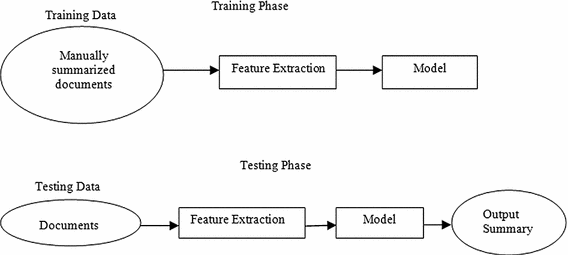
\includegraphics[width=\linewidth]{txtfact.png}
  \caption{Text factorization algorithm}
\end{figure}
\subsubsection{Context-Free Grammar}
It is the grammar that consists rules with a single symbol on the left-hand side of the rewrite rules. Let us create grammar to parse a sentence − “The bird pecks the grains”
Articles (DET) − a | an | the
Nouns − bird | birds | grain | grains
Noun Phrase (NP) − Article + Noun | Article + Adjective + Noun = DET N | DET ADJ N
Verbs − pecks | pecking \ding{120} pecked
Verb Phrase (VP) − NP V \ding{120} V NP
Adjectives (ADJ) − beautiful \ding{120} small \ding{120} chirping

\subsubsection{Feature Extraction}
\begin{itemize}
    \item \textbf{TextBlob} used for part-of-speech tagging, noun phrase extraction, sentiment analysis etc.
    \item Polarity = positivity (-1 to 1), subjectivity (0 to 1, 0 = objective, 1 = subjective).
    \item Polarity of whole sentence, polarities of two parts of sentence, three and four
    \item Helps to assess the change in sentiments throughout the sentence when it is divided into parts
\end{itemize}
\subsection{PUTTY}
\textbf{PUTTY} is a free and open-source terminal emulator, serial console and network file transfer application. It supports several network protocols, including SCP, SSH, Telnet, rlogin, and raw socket connection. It can also connect to a serial port. The name "PuTTY" has no official meaning.
PuTTY was originally written for Microsoft Windows, but it has been ported to various other operating systems. Official ports are available for some Unix-like platforms, with work-in-progress ports to Classic Mac OS and macOS, and unofficial ports have been contributed to platforms such as Symbian, Windows Mobile and Windows Phone.

PuTTY was written and is maintained primarily by Simon Tatham.
\subsubsection{Components of Putty}
PuTTY consists of several components:
\begin{itemize}
    \item PuTTY 
    \par the Telnet, rlogin, and SSH client itself, which can also connect to a serial port
    \item PSCP
    \par an SCP client, i.e. command-line secure file copy. Can also use SFTP to perform transfers
    \item PSFTP
    \par an SFTP client, i.e. general file transfer sessions much like FTP
    \item Plink
    \par a command-line interface to the PuTTY back ends. Usually used for SSH Tunneling
    Pageant: an SSH authentication agent for PuTTY, PSCP and Plink
    \item PuTTYgen
    \par an RSA, DSA, ECDSA and EdDSA key generation utility
    \item pterm
    \par a standalone terminal emulator
\end{itemize}
\subsection{MeaningCloud}
\textbf{MeaningCloud} is a Software as a Service product that enables users to embed text analytics and semantic processing in any application or system. MeaningCloud extends the concept of semantic API with a cloud-based framework that makes the integration of semantic processing into any system something close to a plug-and-play experience. MeaningCloud is available both in SaaS mode and on-premises. MeaningCloud was previously branded as Textalytics.
\subsubsection{Functionalities Of MeaningCloud}
\begin{itemize}
    \item Topic Extraction
    \par identifies appearances of named entities and abstract concepts in the text.
    \item Text Classification
    \par assigns a text to one or several categories in a predefined taxonomy.
    \item Sentiment Analysis
    \par assigns a polarity (positive, negative, neutral) to a document or to the individual topics or attributes appearing in a document (aspect-based sentiment).
    \item Text Clustering
    \par discovers the underlying themes in a document collection and groups these documents according to their similarities and their adherence to those themes.
\end{itemize}
\subsubsection{Integration of MeaningCloud}
\par Advanced APIs provide a functionality optimized for diverse applications and ease of use. In addition, customization and integration capabilities offer a fast learning curve and a short time to obtain results. \par
Customized resource management tools allow users to easily incorporate their own semantic resources (dictionaries, taxonomies, sentiment models) to adapt the operation of the system to their needs.\par 
SDKs and plug-ins increase the convenience and integrability of the APIs in the most common environments and platforms. MeaningCloud provides SDKs for Java, Python, PHP, and Visual Basic, and plug-ins for Microsoft Excel and GATE.
\section{Algorithm Details}
\subsection{Naive Bayes Algorithm}
Using Bayes' theorem, the conditional probability can be decomposed as \newline

\[p {(C_k | x)} =\frac{p{(C_k)}p{(x|C_k)}}{p(x)}\] \newline

In plain English, using Bayesian probability terminology, the above equation can be written as \newline
 
\[ posterior =\frac{prior \times likelihood}{evidence}\]

In practice, there is interest only in the numerator of that fraction, because the denominator does not depend on C and the values of the features Xi are given, so that the denominator is effectively constant. The numerator is equivalent to the joint probability model

\[p ({C_K, X_1,X_2,....,})\]

using the \textbf{chain rule} for repeated applications of the definition of \textbf{conditional probability}

\[p ({C_K, X_1,....,}) = p ({X_1,...,X_n,C_k})\]
= \[p({X_1|X_2,....,X_n,C_k})\hspace{2mm}p(X_2,....,X_n,C_k)\]
=\[p({X_1|X_2,....,X_n,C_k})\hspace{2mm}p({X_2|X_3,....,X_n,C_k})\hspace{2mm}p(X_3,....,X_n,C_k)\]
=\[p({X_1|X_2,....,X_n,C_k})\hspace{2mm}p({X_2|X_3,....,X_n,C_k})...\hspace{2mm}p({X_n-1|X_n,C_k})\hspace{2mm}p(C_k)\]

Now the "naive" \textbf{conditional independence} assumptions come into play: assume that each feature Xi is conditionally independent of every other feature Xj for j =! i, given the category Ck. This means that

\[p ({C_K| X_1,..,X_n})\hspace{2mm} \alpha \hspace{2mm}p({C_k,X_1,....,X_n})\]
=\[p ({C_K}) \hspace{2mm}p{(X_1|C_k)} \hspace{2mm}p{(X_2|C_k)}\hspace{2mm} p{(X_3|C_k)}\]
=\[p ({C_K}) \hspace{2mm}\sum\limits_{i=1}^n \hspace{2mm}p(X_i|C_k)\]

where Alpha denotes \textbf{proportionality}.
\chapter{Software Testing}
\section{Test cases and Test Results}
\begin{table}[H]
\centering
\begin{tabular}{p{0.47in}p{0.79in}p{0.79in}p{-0.18in}p{0.79in}p{1.21in}p{0.88in}p{0.49in}}
\hline
\hline
%row no:1
\multicolumn{1}{|p{0.47in}}{Test Case Id} & 
\multicolumn{1}{|p{0.79in}}{Test Case} & 
\multicolumn{2}{|p{0.79in}}{Objectives} & 
\multicolumn{1}{|p{0.79in}}{Steps} & 
\multicolumn{1}{|p{1.21in}}{Expected Result} & 
\multicolumn{1}{|p{0.88in}}{Actual Result} & 
\multicolumn{1}{|p{0.49in}|}{Test Status} \\
\hline
\hline
%row no:2
\multicolumn{1}{|p{0.47in}}{\begin{tabular}{p{0.47in}}1\\\end{tabular}} & 
\multicolumn{1}{|p{0.79in}}{\begin{tabular}{p{0.50in}}Data Acquisition\\\end{tabular}} & 
\multicolumn{2}{|p{0.79in}}{\begin{tabular}{p{0.60in}}To Connect the Data Feed link and Acquire the live data \\\end{tabular}} & 
\multicolumn{1}{|p{0.79in}}{API Class Object} & 
\multicolumn{1}{|p{1.21in}}{Object Created} & 
\multicolumn{1}{|p{0.88in}}{Object Created} & 
\multicolumn{1}{|p{0.49in}|}{Pass} \\
\hline
\hline
%row no:3
\multicolumn{1}{|p{0.47in}}{} & 
\multicolumn{1}{|p{0.79in}}{} & 
\multicolumn{2}{|p{0.79in}}{} & 
\multicolumn{1}{|p{0.79in}}{API Function Call} & 
\multicolumn{1}{|p{1.21in}}{Function Calling} & 
\multicolumn{1}{|p{0.88in}}{Function Called} & 
\multicolumn{1}{|p{0.49in}|}{Pass} \\
\hline
\hline
%row no:4
\multicolumn{1}{|p{0.47in}}{} & 
\multicolumn{1}{|p{0.79in}}{} & 
\multicolumn{2}{|p{0.79in}}{} & 
\multicolumn{1}{|p{0.79in}}{API Response} & 
\multicolumn{1}{|p{1.21in}}{Response Received} & 
\multicolumn{1}{|p{0.88in}}{Response received from the object} & 
\multicolumn{1}{|p{0.49in}|}{Pass} \\
\hline
\hline
%row no:5
\multicolumn{1}{|p{0.47in}}{} & 
\multicolumn{1}{|p{0.79in}}{} & 
\multicolumn{2}{|p{0.79in}}{} & 
\multicolumn{1}{|p{0.79in}}{Data feed collection} & 
\multicolumn{1}{|p{1.21in}}{All data is collected in runtime object} & 
\multicolumn{1}{|p{0.88in}}{Data collected} & 
\multicolumn{1}{|p{0.49in}|}{Pass} \\
\hline
\hline
%row no:6
\multicolumn{1}{|p{0.47in}}{\begin{tabular}{p{0.47in}}2\\\end{tabular}} & 
\multicolumn{1}{|p{0.79in}}{\multirow{}{}{\begin{tabular}{p{0.79in}}Analysis\\\end{tabular}}} & 
\multicolumn{2}{|p{0.79in}}{\multirow{}{}{\begin{tabular}{p{0.60in}}Check that all the functions are working properly according to plan\\\end{tabular}}} & 
\multicolumn{1}{|p{0.79in}}{Parameters} & 
\multicolumn{1}{|p{1.21in}}{The output should be according to only selected parameters} & 
\multicolumn{1}{|p{0.88in}}{The output is according to selected parameters} & 
\multicolumn{1}{|p{0.49in}|}{Pass} \\
\hline
\hline
%row no:7
\multicolumn{1}{|p{0.47in}}{} & 
\multicolumn{1}{|p{0.79in}}{} & 
\multicolumn{2}{|p{0.79in}}{} & 
\multicolumn{1}{|p{0.79in}}{Invalid Selection} & 
\multicolumn{1}{|p{1.21in}}{If invalid parameter that are not available an error should come} & 
\multicolumn{1}{|p{0.88in}}{Display of error message} & 
\multicolumn{1}{|p{0.49in}|}{Pass} \\
\hline
\hline
%row no:8
\multicolumn{1}{|p{0.47in}}{} & 
\multicolumn{1}{|p{0.79in}}{} & 
\multicolumn{2}{|p{0.79in}}{} & 
\multicolumn{1}{|p{0.79in}}{Erroneous data} & 
\multicolumn{1}{|p{1.21in}}{Discard Erroneous data} & 
\multicolumn{1}{|p{0.88in}}{Erroneous data Discarded} & 
\multicolumn{1}{|p{0.49in}|}{Fail} \\
\hline
\hline
%row no:9
\multicolumn{1}{|p{0.47in}}{} & 
\multicolumn{1}{|p{0.79in}}{} & 
\multicolumn{2}{|p{0.79in}}{} & 
\multicolumn{1}{|p{0.79in}}{Historical data} & 
\multicolumn{1}{|p{1.21in}}{Collect all the Historical Prices} & 
\multicolumn{1}{|p{0.88in}}{Data Collected} & 
\multicolumn{1}{|p{0.49in}|}{Pass} \\
\hline
\hline
\end{tabular}
\caption{Test case 1}
\end{table}
%%%%%%%%%%%%%%%%%%%% Table No: 2 starts here %%%%%%%%%%%%%%%%%%%%
\begin{table}[H]
\centering
\begin{tabular}{p{0.45in}p{0.77in}p{0.85in}p{0.77in}p{1.2in}p{0.94in}p{0.45in}}
\hline
\hline
\multicolumn{1}{|p{0.45in}}{3} & 
\multicolumn{1}{|p{0.77in}}{System} & 
\multicolumn{1}{|p{0.85in}}{Check\ that the systems performance does  not degrade} & 
\multicolumn{1}{|p{0.77in}}{Performance} & 
\multicolumn{1}{|p{1.2in}}{System performance should not degrade} & 
\multicolumn{1}{|p{0.94in}}{System performance does not degrade} & 
\multicolumn{1}{|p{0.40in}|}{Pass} \\
\hline
\hline
%row no:1
\multicolumn{1}{|p{0.45in}}{\multirow{}{}{\begin{tabular}{p{0.40in}}4\\\end{tabular}}} & 
\multicolumn{1}{|p{0.90in}}{\multirow{}{}{\begin{tabular}{p{0.75in}}Application\\\end{tabular}}} & 
\multicolumn{1}{|p{0.85in}}{\multirow{}{}{\begin{tabular}{p{0.75in}}Check that the application works properly with all system configuration and response time must not degrade\\\end{tabular}}} & 
\multicolumn{1}{|p{0.77in}}{Generation of forecasting} & 
\multicolumn{1}{|p{1.2in}}{forecasting generation should be done within minimum expected time.} & 
\multicolumn{1}{|p{0.94in}}{The output is in time limit.} & 
\multicolumn{1}{|p{0.45in}|}{Pass} \\
\hline
\hline
%row no:2
\multicolumn{1}{|p{0.45in}}{} & 
\multicolumn{1}{|p{0.77in}}{} & 
\multicolumn{1}{|p{0.80in}}{} & 
\multicolumn{1}{|p{0.75in}}{Adding new data} & 
\multicolumn{1}{|p{1.2in}}{Data entered by hospital managers should not take more than expected time to upload.} & 
\multicolumn{1}{|p{0.80in}}{Data is uploaded in the expected time range} & 
\multicolumn{1}{|p{0.45in}|}{Pass} \\
\hline
\hline
%row no:3
\multicolumn{1}{|p{0.45in}}{} & 
\multicolumn{1}{|p{0.77in}}{} & 
\multicolumn{1}{|p{0.85in}}{} & 
\multicolumn{1}{|p{0.77in}}{Values displayed on screen} & 
\multicolumn{1}{|p{1.2in}}{The values displayed after analysis should be correct.} & 
\multicolumn{1}{|p{0.94in}}{The values are correctly displayed} & 
\multicolumn{1}{|p{0.45in}|}{Pass} \\
\hline
\hline%row no:4
\multicolumn{1}{|p{0.45in}}{\begin{tabular}{p{0.45in}}5\\\end{tabular}} & 
\multicolumn{1}{|p{0.77in}}{\begin{tabular}{p{0.77in}}Database\\\end{tabular}} & 
\multicolumn{1}{|p{0.85in}}{\begin{tabular}{p{0.75in}}Proper database queries are fired on the database according to the Fake and historical data\\\end{tabular}} & 
\multicolumn{1}{|p{0.77in}}{Retrieval of tweets information} & 
\multicolumn{1}{|p{1.2in}}{Should provide proper authentication} & 
\multicolumn{1}{|p{0.90in}}{Authentication is provided} & 
\multicolumn{1}{|p{0.45in}|}{Pass} \\
\hline
\hline
%row no:5
\multicolumn{1}{|p{0.45in}}{} & 
\multicolumn{1}{|p{0.77in}}{} & 
\multicolumn{1}{|p{0.85in}}{} & 
\multicolumn{1}{|p{0.77in}}{Update} & 
\multicolumn{1}{|p{1.2in}}{Whenever\ new accounts are created or  data is added ,it should be reflected in the database. \par } & 
\multicolumn{1}{|p{0.94in}}{Updates are reflected in database.} & 
\multicolumn{1}{|p{0.45in}|}{Pass} \\
\hline
\hline
\end{tabular}
\caption{Test case 2}
\end{table}
\chapter{Results}
\section{Screen Shots}
\begin{figure}[h!]
  \centering
  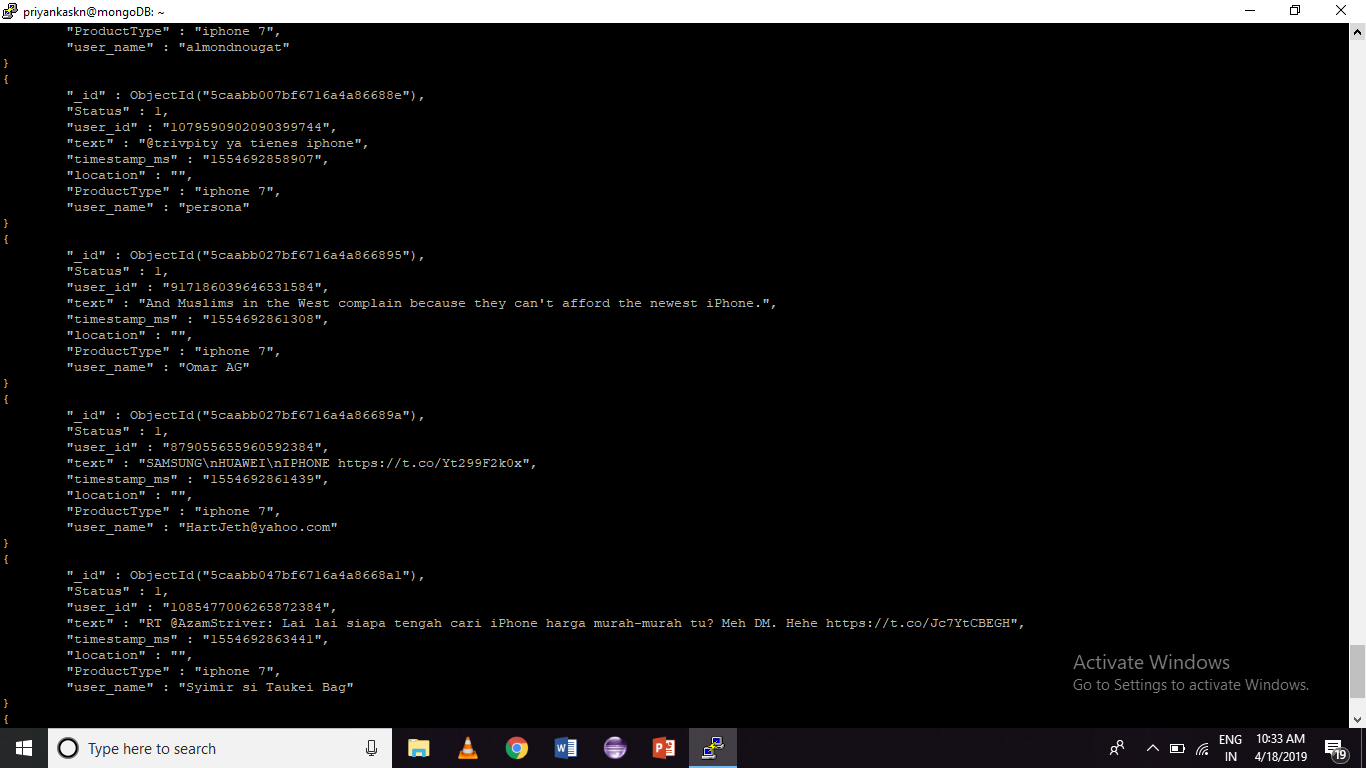
\includegraphics[width=\linewidth]{mod1.png}
  \caption{Module 1: Data acquisition and data preprocessing}
\end{figure}

\begin{figure}[h!]
  \centering
  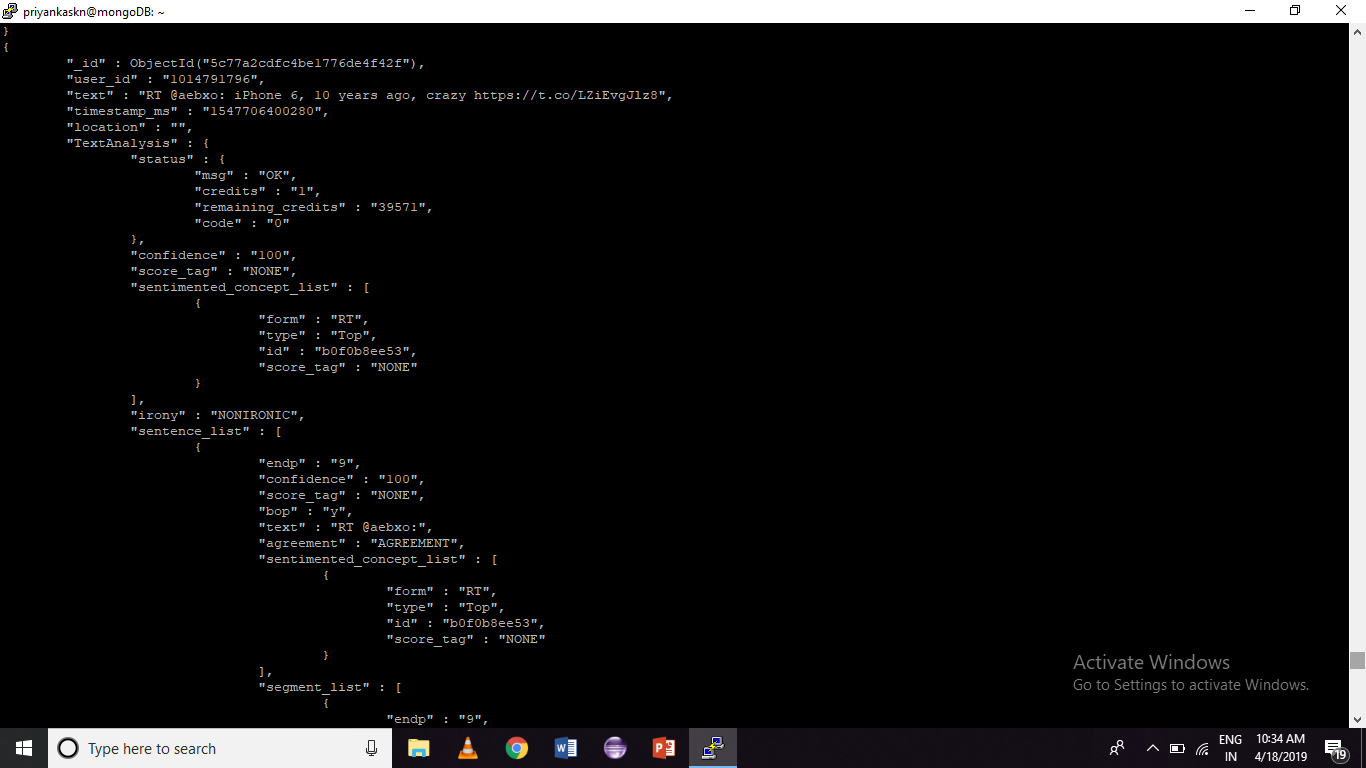
\includegraphics[width=\linewidth]{mod2.png}
  \caption{Module 2: Text analysis}
\end{figure}

\begin{figure}[h!]
  \centering
  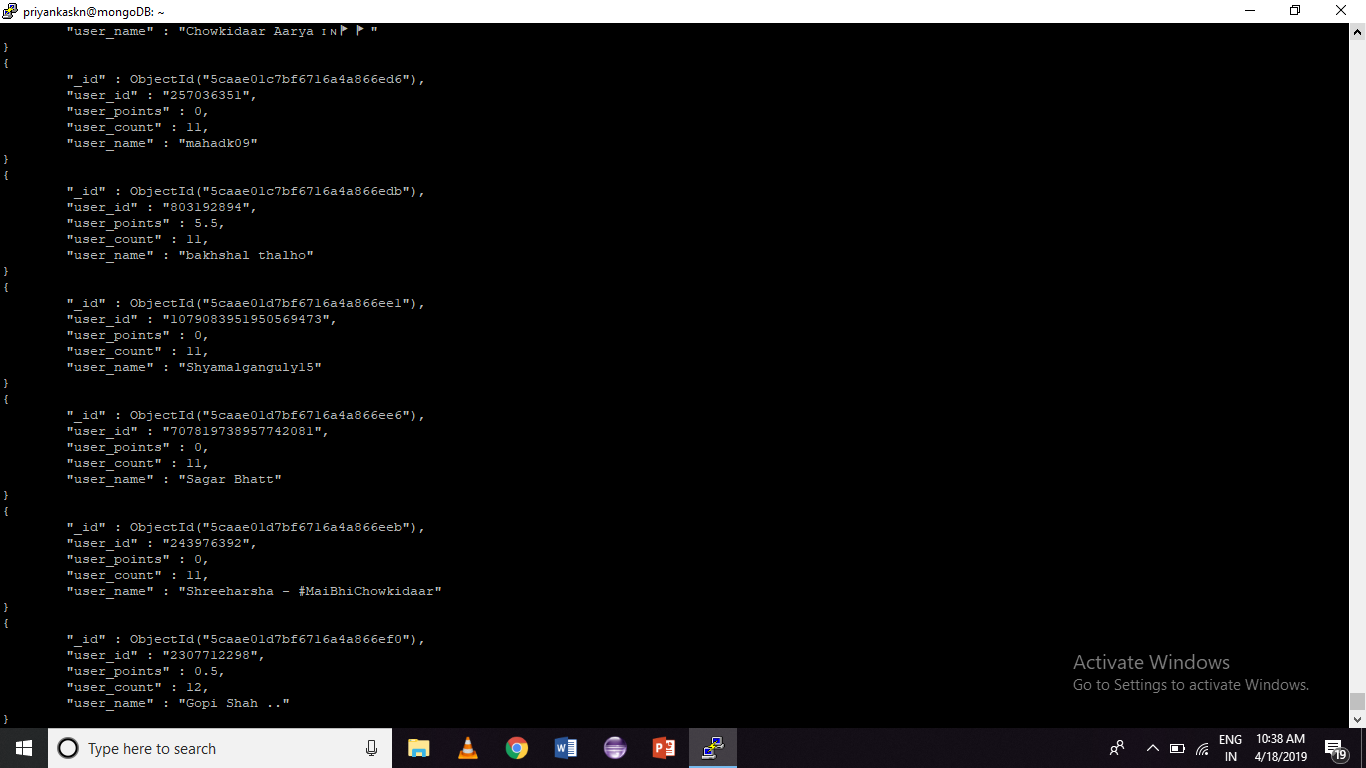
\includegraphics[width=\linewidth]{mod3.png}
  \caption{Module 3: User reviews classification}
\end{figure}

\begin{figure}[h!]
  \centering
  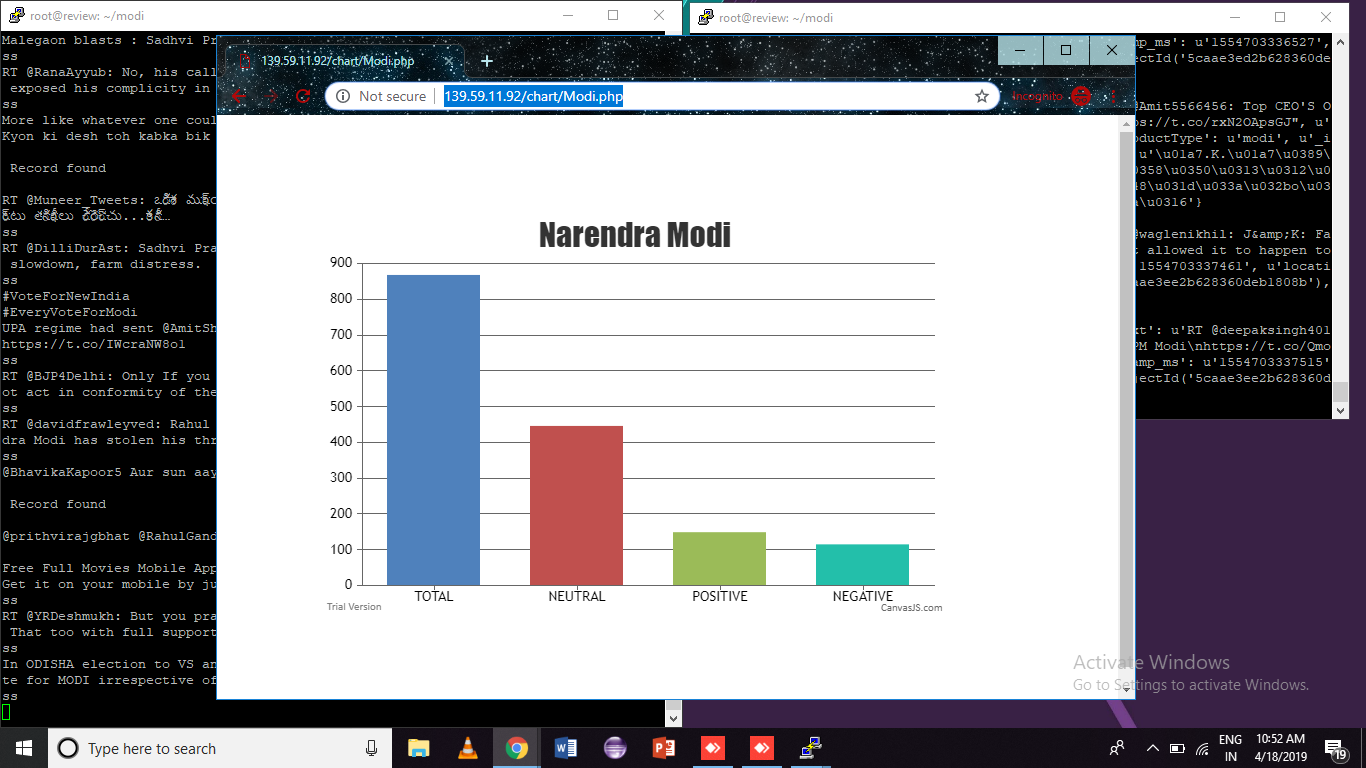
\includegraphics[width=\linewidth]{modres.png}
  \caption{Module 4: Review graph}
\end{figure}
\newpage
\chapter{Conclusions}
\section{Conclusions}
Sarcasm is a complex phenomenon. In this project, it is noticed how real time dataset can act as huge asset in terms of data gathering and how a few basic features
like punctuation can be powerful in the detection (accuracy) of sophisticated language
form like that of sarcasm. Data pre-processing and feature engineering would be one of
the most important tasks in terms of improving accuracy and more in-depth analysis in
these domains will help in improving the accuracy considerably.
\section{Future Work}
In the above section as mentioned few improvements that can be incorporated in the
feature set that has been used. Apart from these it can include topic based feature set.
Other major improvement that can be done is in data processing. Spell checks, word
sense disambiguation, slang detection can make the data more cleaner and can help in
better classification. Also, the ratio of the sarcastic to non sarcastic data is quiet high
which is not the case in the real word hence there is a need to gather more data with lower ratio 
to get the real performance measure of our system
\section{Applications}
\begin{itemize}
    \item Will be beneficial for E-Commerce websites ass they can take decisions according our analysis.
    \item Organizations. 
    \item Schools and colleges-While taking admissions in a school or college better to check sarcasm analysis first.
    \item Private sectors-Companies sarcasm reviews will be considered.
\end{itemize}
\newpage
\appendix
\section{APPENDIX A}
\textbf{Feasibility} 
\par 
Feasibility study is done to determine project success ratio that means to see whether the project will be useful or not. It determines all positive and negative points of project to test success ratio. There are various types of feasibility study as follows:
\begin{itemize}
    \item Technical Feasibility
    The development process of E-Commerce System with Chatbot for product recommendation would be advantageous as the technologies and tools required for development are available on the internet to use. Languages and tools required for developing website are HTML, CSS, JavaScript, JQuery, Bootstrap, Spring and MySQL database. The three important parts of developing chatbots are messaging platform, API to design Bot Logic with Machine Learning and actions to be taken should be defined.
    \item Operational Feasibility
    The Proposed System is intended to provide a very user-friendly and easy to use interface which will be beneficial for both the customers and the administrator team. This system would be easily accessible among the customers, as there is no need of any special skill set for using the application. This system also benefits the users as they do not have to download anything on their terminals increasing their efficiency and ease of use.
    \item Safety Feasibility
    The customers need to login to the system to observe their order and search history for product recommendation. So it is necessary to store customers’ credentials securely at the server. Also it is mandatory to store each customer’s history separately in organized way to gain customer insight.
    \item Scheduled Feasibility
    Projects are always given deadlines. Every project is completed in a specific duration. We have the project duration of six months only. So we will try our level best to fulfil each and every requirement. We have to complete the project in time and if it is not possible to complete the software in time then we would try our best to fulfil requirements.
    \item Economic Feasibility
    The E-commerce system with chatbots has a low development cost. The low cost is attributed to the usage of the existing resources of the department related to sellers and technologies required to develop a chatbot. As these resources are available online along with tutorials, it will require less development cost. As the website is very user friendly and easy to use, there is no need to provide special training to the users of the website, thus saving valuable time and money.
\end{itemize}
\textbf{Mathematical Model}\\
Set Theory Analysis:
\begin{itemize}
    \item Let ‘S’ be the | Error detection in big data as the final set\\
S = {empty set} 
\item Identify the inputs as D\\
S = {D, …}
D = {D1, D2, D3, D4| ‘D’ given Data files}

\item Identify the outputs as O\\
S = {D, L, A…}
D = {D1, D2, D3, D4| ‘D’ gives data files}
L = {L1, L2 …| ‘L’ gives the log files for upload and download and repair}
A = {A1, A2, A3,… | ‘A’ gives alerts }

\item Identify the functions as ‘F’\\
S = {D, L, A, F…}
F = {F1(), F2(), F3(), F4(), F5(), F6() }
\end{itemize}
F1 (V): Upload
F2 (V): integrity check 
F3 (V): Log generation
F4 ( T ) :: Sarcasam Detection
F4 ( D ) :: Restore the file
F6 ( V ) :: Download the data file

Hence the functionality can be shown as,
\begin{figure}[h!]
  \centering
  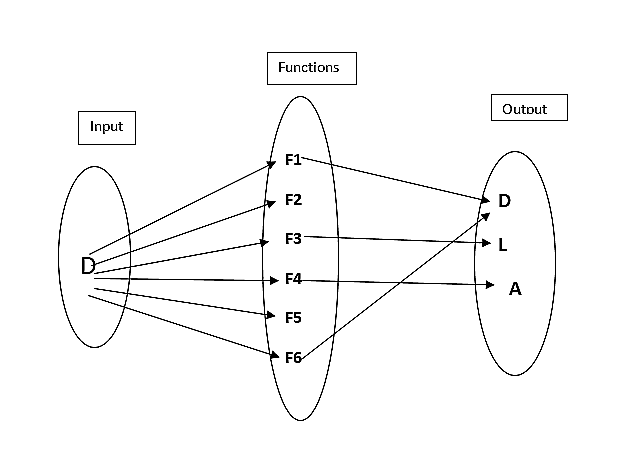
\includegraphics[height=10cm, width=10cm]{math.png}
  \caption{Mathematical model}
\end{figure}
\newpage
\section{APPENDIX B}
\textbf{Details of the Publication}
\newline
\textbf{Name of the publication} : \par International Conference on Internet of Things, Next Generation Networks and Cloud Computing 2019
\newline
\textbf{Review} :\par The idea is well stated but detailed literature review need to be improved, also proposed system and result section need to be elaborated in detail. Bifurcation between existing system and given model is not that much clear.
\newpage
\textbf{Certificate}
\begin{figure}[h!]
  \centering
  
\includegraphics[width=\linewidth]{cert.jpg}
  \caption{ICINC certificate}
\end{figure}
\newpage
\textbf{Paper}
\newline
\begin{center}
 \textbf{Sarcasm Detection Using Text Factorization on Reviews}

Mayuri Patil1, Priyanka Lodhe2, Vijaya Dabade3, Tejaswini Murudkar4, Shailesh Patil5
1,2,3,4 Student, Smt. Kashibai Navale College of Engineering
5Assistant Professor, Smt. Kashibai Navale College of Engineering
Email: mayuripatil733@gmail.com, priyankalodhe09@gmail.com,  vijayadabade105@gmail.com, tejum14320@gmail.com, shaileshpp19@gmail.com 
\end{center}
 
\textbf{ABSTRACT} \par The research area of sentiment analysis, opinion mining, sentiment mining and sentiment extraction has gained popularity in the last years. Online reviews are becoming very important criteria in measuring the quality of a business. This paper presents a sentiment analysis approach to business reviews classification using a large reviews dataset provided by Yelp: Yelp Challenge dataset. In this work, we propose several approaches for automatic sentiment classification, using two feature extraction methods and four machine learning models. It is illustrated a comparative study on the effectiveness of the ensemble methods for reviews sentiment classification.

\textbf{INTRODUCTION}
\par
Sentiment analysis has become an important research area for understanding people’s opinion on a matter by analyzing a large amount of information. The active feedback of the people is valuable not only for companies to analyze their customers’ satisfaction and the monitoring of competitors, but is also very useful for consumers who want to research a product or a service prior to making a purchase. 

\textbf{MOTIVATION}
\par
With the increased amount of data collection taking place as a result of social media interaction, scientific experiments, and even e-commerce applications, the nature of data it has been evolving. As a result of this data generation from many different sources, “new generation” data, presents challenges as it is not all relational and lacks predefined structures. In this project, the aim is try to sort these issues and provide a way for better acquisition and processing of this type of data. The aim will be Analyzing the real time social network data and try to eliminate the Fake reviews and analyze the sarcasm in it.

\textbf{STATE OF ART}
\par
Mondher Bouazizi and Tomoaki Ohtsuki [1] explained- use of Part-of-Speech-tags to extract patterns characterizing the level of sarcasm of tweets training set since the number of patterns we extracted from the current one is 346 541

Mondher Bouazizi and Tomoaki Ohtsuki [2]
 analyzed- ran the classification using the classifiers “Random Forest”, “Support Vector Machine” (SVM), “k Nearest Neighbors” (k-NN) and “Maximum Entropy”.

Huaxun Deng, Linfeng Zhao et al. [3] analyzed - used the similarity characteristics of the text to determine a set of true negative cases or fake reviews and extract the characteristic vector from multiple aspects. Then, take the technique of K-Means to cluster towards the comments. it label the comments as the negative case if the comments is close to the true negative cases, whereas label the comments as the positive case if the comment far away from the trusted negative case

Shalini Raghav, Ela Kumar [4] explained- have identified pattern extraction, hashtag based and contextual approach.

Tanya Jain, Nilesh Agrawal et al. [5] analyzed- Problem of sarcasm positive sentiments attached to a negative situation. The work uses two approaches- voted classifier and random forest classifier. And in the proposed model they used seeding algorithm and pragmatic classifier to detect emoticon based sarcasm.

Edwin Lunando, Ayu Purwarianti [6] analyzed- To solve the high computational overhead and low classification efficiency of the KNN algorithm, a text feature vector representation method based on information gain and non-negative matrix factorization is proposed.


\textbf{GAP ANALYSIS}
\par
The process of detecting sarcasm was done on the basis of fixed dataset. The dataset was saved and then the further processing started. The dataset was or could be manipulated easily as it used to be stored. Whereas in our process of detecting sarcasm, the detection  is done on real time data. The data is not saved permanently. The minute you refresh the data would be refreshed from the memory, i.e. new data would be shown. The data would be only saved temporarily. Temporary storage would be done through MongoDB. As the data is not being saved, manipulation of the data is impossible. And the results are more accurate and unbiased. 

\textbf{PROPOSED WORK}
\par
The increase in the data rates generated on the digital universe is escalating exponentially. With a view in employing current tools and technologies to analyze and store, a massive volume of data are not up to the mark, since they are unable to extract required sample data sets. Therefore, the goal is to design an architectural platform for analyzing both remote access real time and offline data. When a business enterprise can pull-out all the useful information obtainable in the Big Data rather than a sample of its data set, in that case, it has an influential benefit over the market competitors. Big Data analytics helps us to gain insight and make better decisions. Therefore, with the intentions of using Big Data, modifications in paradigms are at utmost. To support our motivations,the need to describe some areas where Big Data can play an important role. In healthcare scenarios, medical practitioners gather massive volume of data about patients, medical history, medications, and other details. The above-mentioned data are accumulated in drug-manufacturing companies. The nature of these data is very complex, and sometimes the practitioners are unable to show a relationship with other information, which results in missing of important information. With a view in employing advance analytic techniques for organizing and extracting useful information from Big Data results in personalized medication, the advance Big Data analytic techniques give insight into hereditary causes of the disease. In the Same way data is also generated for the reviews of the product across various services but sometimes we have to differentiate between fake reviews and Genuine Reviews for the input of our decision making process in Business.

\textbf{CONCLUSION AND FUTURE WORK}
\par
\textbf{Conclusion}
\par Sarcasm is a complex phenomenon. In this project, it has been noticed how real time dataset can act as huge asset in terms of data gathering and how a few basic features like punctuation can be powerful in the detection (accuracy) of sophisticated language form like that of sarcasm. Data pre-processing and feature engineering would be one of the most important tasks in terms of improving accuracy and more in-depth analysis in these domains will help in improving the accuracy considerably. The goal of the system is to efficient detect sarcasm into positive, negative and neutral categories. Not just detecting the sarcasm but also detecting reviews in positive, negative and neutral categories in the form of a graphical representation.

\textbf{Future Work}
\par
	In the above section, as mentioned few improvements that can be incorporated in the feature set that have been used. Also, the ratio of the sarcastic to non-sarcastic data is quiet high which is not the case in the real word hence the need to gather more data with lower ratio to get the real performance measure of our system. So basically, with detecting the sarcasm it will also be looking for foul languages and detecting them in the reviews the data wouldn’t be saved and hence there is no scope of manipulation of the data. The results will be pretty unbiased. The goal is to not just limit it to the reviews, but to add  this process in comments as well.
\newpage
\section{APPENDIX C}
\textbf{PLAGARISM REPORT}
\begin{figure}[h!]
  \centering
  %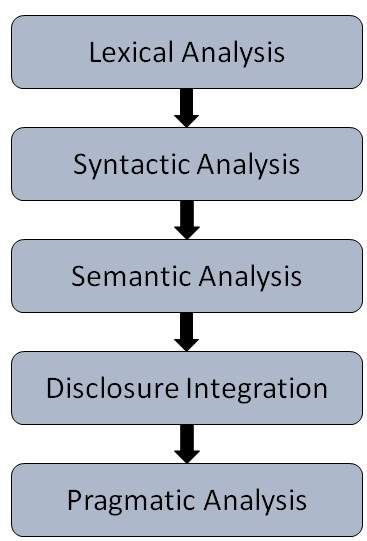
\includegraphics[width=\linewidth]{nlpstep.png}
  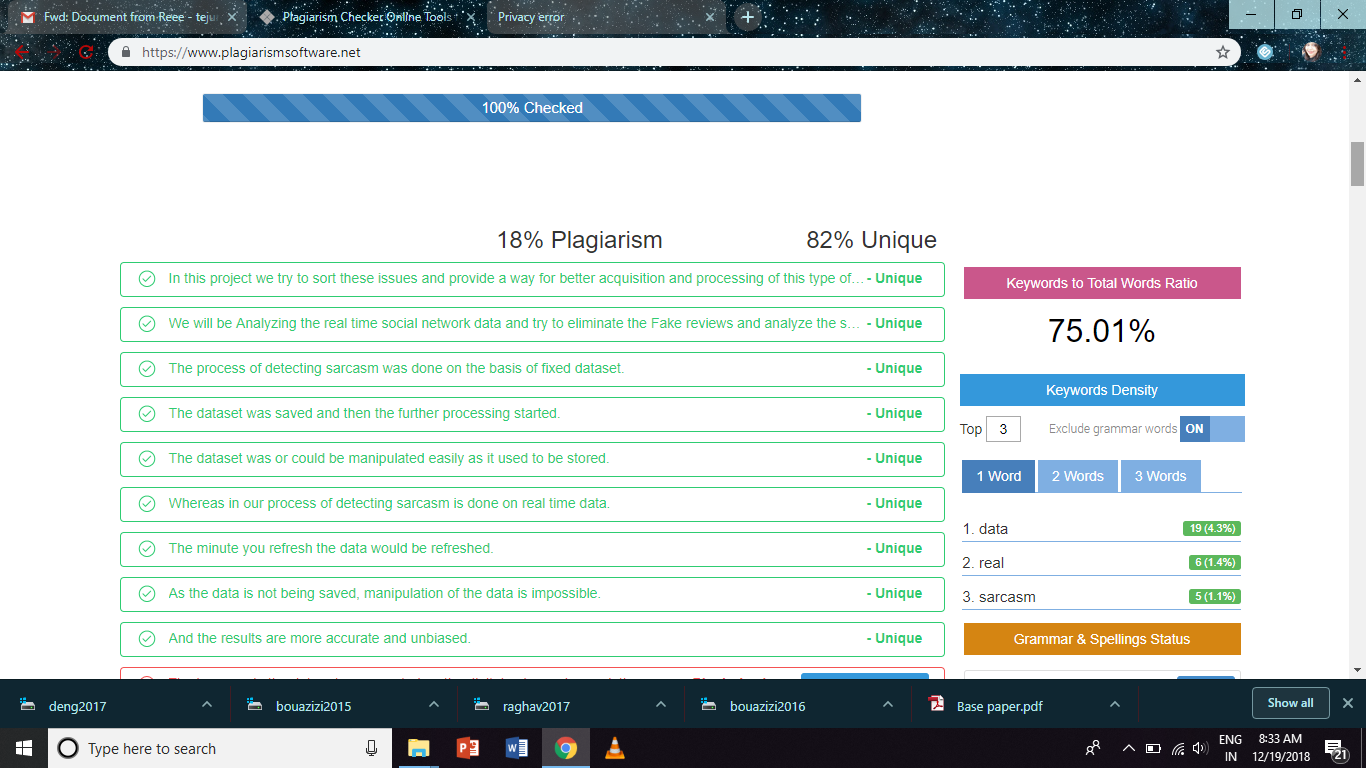
\includegraphics[
  width=13cm,
  height=10cm,
]{plag.png}
  \caption{Plagarism report}
\end{figure}
\newpage
\begin{thebibliography}{99}
 
\bibitem{} Mondher Bouazizi, Tomoaki Ohtsuki \textquotedblleft Sarcasm Detection in Twitter(2015)\textquotedblright\
\bibitem{} Mondher Bouazizi, Tomoaki Ohtsuki \textquotedblleft A Pattern-Based Approach for Sarcasm Detection on Twitter(2016)\textquotedblright\

\bibitem{} Huaxun Deng, Linfeng Zhao, Ning Luo, Yuan Liu*, Guibing Guo, Xingwei Wang, Zhenhua Tan, Shuang Wang and Fucai Zhou \textquotedblleft Semi-supervised Learning based Fake Review Detection(2017)\textquotedblright\

\bibitem{} Shalini Raghav, Ela Kumar\textquotedblleft Review of Automatic Sarcasm Detection(2017 review paper)\textquotedblright\

\bibitem{} Tanya Jain,Nilesh Agrawal,Garima Goyal,Niyati Aggrawal\textquotedblleft Sarcasm Detection of Tweets: A comparative Study(2017)\textquotedblright\

\bibitem{} Edwin Lunando,Ayu Purwarianti\textquotedblleft Indonesian Social Media Sentiment Analysis with Sarcasm Detection(2013)\textquotedblright\

\bibitem{} Yongxia Jing, Heping Gou,Chuanyi Fu,Qiang Liu\textquotedblleft Text Classification Algorithm Based on Non-negative Matrix Factorization(2017)\textquotedblright\

\bibitem{} Tanvir Ahmad, Halima Akhtar, Akshay Chopra, Mohd Waris\textquotedblleft Satire Detection from Web Documents using machine Learning Methods(2014)\textquotedblright\

\bibitem{}Paras Dharwal,Tanupriya Choudhury,Rajat Mittal,Paveen Kumar \textquotedblleft Automatic Sarcasm Detection using feature selection(2017)\textquotedblright\

\bibitem{} Manoj Y. Manohar,Prof. Pallavi Kulkarni\textquotedblleft Improvement Sarcasm Analysis using NLP and Corpus based Approach(2017)\textquotedblright\

\bibitem{}  Anukarsh G Prasad, Sanjana S, Skanda M Bhat, B S Harish \textquotedblleft Sentiment Analysis for Sarcasm Detection on Streaming Short Text Data(2017)\textquotedblright\

\bibitem{} A, Esuli and F. Sebastiani, "SentiWordNet: A Publicly Available Lexical Resource for Opinion Mining(2006)\textquotedblright\

\bibitem{} T. Wilson, J. Wiebe and P
polarity in phrase-level sentiment
Human Language Technology(2005)

\bibitem{} R. McDonald, T. Neylon, G. Reis,
entiment Summarizer for Local Service
W Workshop on NLP Challenges in the
LPIX, 2008
\bibitem{} Hoffmann "Recognizing contextual
nt analysis", Proc. of the conference on
and Empirical Methods in NLP, 2005
\end{thebibliography}
\end{document}
